% This LaTeX was auto-generated from MATLAB code.
% To make changes, update the MATLAB code and export to LaTeX again.

\documentclass{article}

\usepackage[utf8]{inputenc}
\usepackage[T1]{fontenc}
\usepackage{lmodern}
\usepackage{graphicx}
\usepackage{color}
\usepackage{hyperref}
\usepackage{amsmath}
\usepackage{amsfonts}
\usepackage{epstopdf}
\usepackage[table]{xcolor}
\usepackage{matlab}

\sloppy
\epstopdfsetup{outdir=./}
\graphicspath{ {./signal_based_live_images/} }

\matlabhastoc

\begin{document}

\label{T_C40A9D76}
\matlabtitle{Signal Based PM}

\matlabtableofcontents{Table of Contents}
\label{H_CE02C3B4}
\matlabheading{Introduction}

\begin{par}
\begin{flushleft}
Before the final solution was developed in the whole dataset, the smaller reduced dataset was used for experiments and planning algorithms. 
\end{flushleft}
\end{par}

\label{H_3084775A}
\matlabheading{Import datastore}

\begin{par}
\begin{flushleft}
Full datastore contain 4840 members. Each member has information from one mesurement, and extracted features from all signals:
\end{flushleft}
\end{par}

\begin{enumerate}
\setlength{\itemsep}{-1ex}
   \item{\begin{flushleft} Measured signals \end{flushleft}}
   \item{\begin{flushleft} Setting parameters (valves, dampers, load) \end{flushleft}}
   \item{\begin{flushleft} Power spectum calculated from measured signals \end{flushleft}}
   \item{\begin{flushleft} Statistical and Frequency features extracted from signals \end{flushleft}}
\end{enumerate}

\begin{par}
\begin{flushleft}
From every signal in dataset statistical features were calculated. Using Welch's power spectral density estimation frequency features were calculated too. 
\end{flushleft}
\end{par}

\begin{par}
\begin{flushleft}
Original dataset contain 6 large .mat files. Those files was devided to members, for better memory perfomance during the feature extraction and writing output to files back.
\end{flushleft}
\end{par}

\begin{matlabcode}
clc; clear all; close all;
has_data = false;
if has_data
    run import_full_datastore.m
    datastore 
end  
\end{matlabcode}

\begin{par}
\begin{flushleft}
Datastore handler functions \textit{readData }and \textit{writeData }were coded with respect to members.
\end{flushleft}
\end{par}


\vspace{1em}

\label{H_F55D877D}
\matlabheading{Data exploration}

\begin{par}
\begin{flushleft}
There are types of sensors:
\end{flushleft}
\end{par}

\begin{enumerate}
\setlength{\itemsep}{-1ex}
   \item{\begin{flushleft} Linear encoder \end{flushleft}}
   \item{\begin{flushleft} Flow sensor \end{flushleft}}
   \item{\begin{flushleft} Pressure sensor \end{flushleft}}
   \item{\begin{flushleft} Temperature sensor \end{flushleft}}
   \item{\begin{flushleft} Accelerometer \end{flushleft}}
   \item{\begin{flushleft} Strain gauge \end{flushleft}}
   \item{\begin{flushleft} Microphones \end{flushleft}}
   \item{\begin{flushleft} Proximity sensors \end{flushleft}}
\end{enumerate}

\begin{par}
\begin{flushleft}
The whole dataset was divided into 20 Labels by place of fault accumulate: 
\end{flushleft}
\end{par}

\begin{enumerate}
\setlength{\itemsep}{-1ex}
   \item{\begin{flushleft} Healthy \end{flushleft}}
   \item{\begin{flushleft} Throlette valve 1 \end{flushleft}}
   \item{\begin{flushleft} Throlette valve 2  \end{flushleft}}
   \item{\begin{flushleft} Small damper bottom \end{flushleft}}
   \item{\begin{flushleft} Small damper upper \end{flushleft}}
   \item{\begin{flushleft} Large dampers  \end{flushleft}}
   \item{\begin{flushleft} And combinations of these faults \end{flushleft}}
\end{enumerate}

\begin{matlabcode}
addpath("scripts/");
data_test = load("data_test/data10_1_1.mat").data
\end{matlabcode}
\begin{matlabtableoutput}
{
\begin{tabular} {|c|c|c|c|c|c|c|c|c|c|c|c|c|c|c|c|c|c|c|c|c|c|c|c|c|c|c|c|c|c|c|c|c|c|c|c|c|c|c|c|c|c|c|c|c|c|c|c|c|c|c|c|c|c|c|c|c|c|c|c|c|c|c|c|c|c|c|}\hline
\mlcell{ } & \mlcell{FlowExtrusion} & \mlcell{FlowContraction} & \mlcell{AirPressure} & \mlcell{AccelerometerMoving\_axisY} & \mlcell{AccelerometerMoving\_axisZ} & \mlcell{AccelerometerStatic\_axisY} & \mlcell{AccelerometerStatic\_axisZ} & \mlcell{StrainGauge} & \mlcell{ProximitySensor\_bottom} & \mlcell{ProximitySensor\_upper} & \mlcell{LeverPosition} & \mlcell{MIC\_uBumper} & \mlcell{MIC\_bBumper} & \mlcell{MIC\_Ambient} & \mlcell{Temp\_Cylinder} & \mlcell{Temp\_Ambient} & \mlcell{outValveHP} & \mlcell{outValveWP} & \mlcell{FaultCode} & \mlcell{Settings.Load} & \mlcell{ThrottleValve1} & \mlcell{ThrottleValve2} & \mlcell{SmallDamper\_upper} & \mlcell{LargeDamper\_upper} & \mlcell{SmallDamper\_bottom} & \mlcell{LargeDamper\_bottom} & \mlcell{Label} & \mlcell{LeverPosition\_stats} & \mlcell{LeverVelocity} & \mlcell{LeverPosition\_ps} & \mlcell{LeverVelocity\_stats} & \mlcell{MIC\_uBumper\_stats} & \mlcell{MIC\_bBumper\_stats} & \mlcell{MIC\_Ambient\_stats} & \mlcell{MIC\_uBumper\_ps} & \mlcell{MIC\_bBumper\_ps} & \mlcell{MIC\_Ambient\_ps} & \mlcell{MIC\_bBumper\_ps\_spec} & \mlcell{MIC\_Ambient\_ps\_spec} & \mlcell{MIC\_uBumper\_ps\_spec} & \mlcell{FlowContraction\_stats} & \mlcell{FlowExtrusion\_stats} & \mlcell{FlowContraction\_ps} & \mlcell{FlowExtrusion\_ps} & \mlcell{FlowContraction\_ps\_spec} & \mlcell{FlowExtrusion\_ps\_spec} & \mlcell{AccelerometerMoving\_axisY\_stats} & \mlcell{AccelerometerMoving\_axisZ\_stats} & \mlcell{AccelerometerStatic\_axisY\_stats} & \mlcell{AccelerometerStatic\_axisZ\_stats} & \mlcell{AccelerometerMoving\_axisY\_ps} & \mlcell{AccelerometerMoving\_axisZ\_ps} & \mlcell{AccelerometerStatic\_axisY\_ps} & \mlcell{AccelerometerStatic\_axisZ\_ps} & \mlcell{AccelerometerMoving\_axisY\_ps\_spec} & \mlcell{AccelerometerMoving\_axisZ\_ps\_spec} & \mlcell{AccelerometerStatic\_axisY\_ps\_spec} & \mlcell{AccelerometerStatic\_axisZ\_ps\_spec} & \mlcell{StrainGauge\_stats} & \mlcell{StrainGauge\_ps} & \mlcell{StrainGauge\_ps\_spec} & \mlcell{ProximitySensor\_bottom\_stats} & \mlcell{ProximitySensor\_upper\_stats} & \mlcell{AirPressure\_stats} & \mlcell{AirPressure\_ps} & \mlcell{AirPressure\_ps\_spec} \\ \hline
\mlcell{1} & \mlcell{10000x1 timetable} & \mlcell{10000x1 timetable} & \mlcell{10000x1 timetable} & \mlcell{10000x1 timetable} & \mlcell{10000x1 timetable} & \mlcell{10000x1 timetable} & \mlcell{10000x1 timetable} & \mlcell{10000x1 timetable} & \mlcell{10000x1 timetable} & \mlcell{10000x1 timetable} & \mlcell{10000x1 timetable} & \mlcell{400000x1 timetable} & \mlcell{400000x1 timetable} & \mlcell{400000x1 timetable} & \mlcell{1x1 timetable} & \mlcell{1x1 timetable} & \mlcell{10000x1 timetable} & \mlcell{10000x1 timetable} & \mlcell{1x1 table} & \mlcell{1x1 table} & \mlcell{1x1 table} & \mlcell{1x1 table} & \mlcell{1x1 table} & \mlcell{1x1 table} & \mlcell{1x1 table} & \mlcell{1x1 table} & \mlcell{"health"} & \mlcell{1x13 table} & \mlcell{10000x1 timetable} & \mlcell{2049x2 table} & \mlcell{1x13 table} & \mlcell{1x13 table} & \mlcell{1x13 table} & \mlcell{1x13 table} & \mlcell{65537x2 table} & \mlcell{65537x2 table} & \mlcell{65537x2 table} & \mlcell{1x21 table} & \mlcell{1x21 table} & \mlcell{1x21 table} & \mlcell{1x13 table} & \mlcell{1x13 table} & \mlcell{2049x2 table} & \mlcell{2049x2 table} & \mlcell{1x11 table} & \mlcell{1x11 table} & \mlcell{1x13 table} & \mlcell{1x13 table} & \mlcell{1x13 table} & \mlcell{1x13 table} & \mlcell{2049x2 table} & \mlcell{2049x2 table} & \mlcell{2049x2 table} & \mlcell{2049x2 table} & \mlcell{1x21 table} & \mlcell{1x21 table} & \mlcell{1x21 table} & \mlcell{1x21 table} & \mlcell{1x13 table} & \mlcell{2049x2 table} & \mlcell{1x21 table} & \mlcell{1x13 table} & \mlcell{1x13 table} & \mlcell{1x13 table} & \mlcell{2049x2 table} & \mlcell{1x21 table} \\ 
\hline
\end{tabular}
}
\end{matlabtableoutput}
\begin{matlabcode}
data_plot(data_test)
\end{matlabcode}
\begin{center}
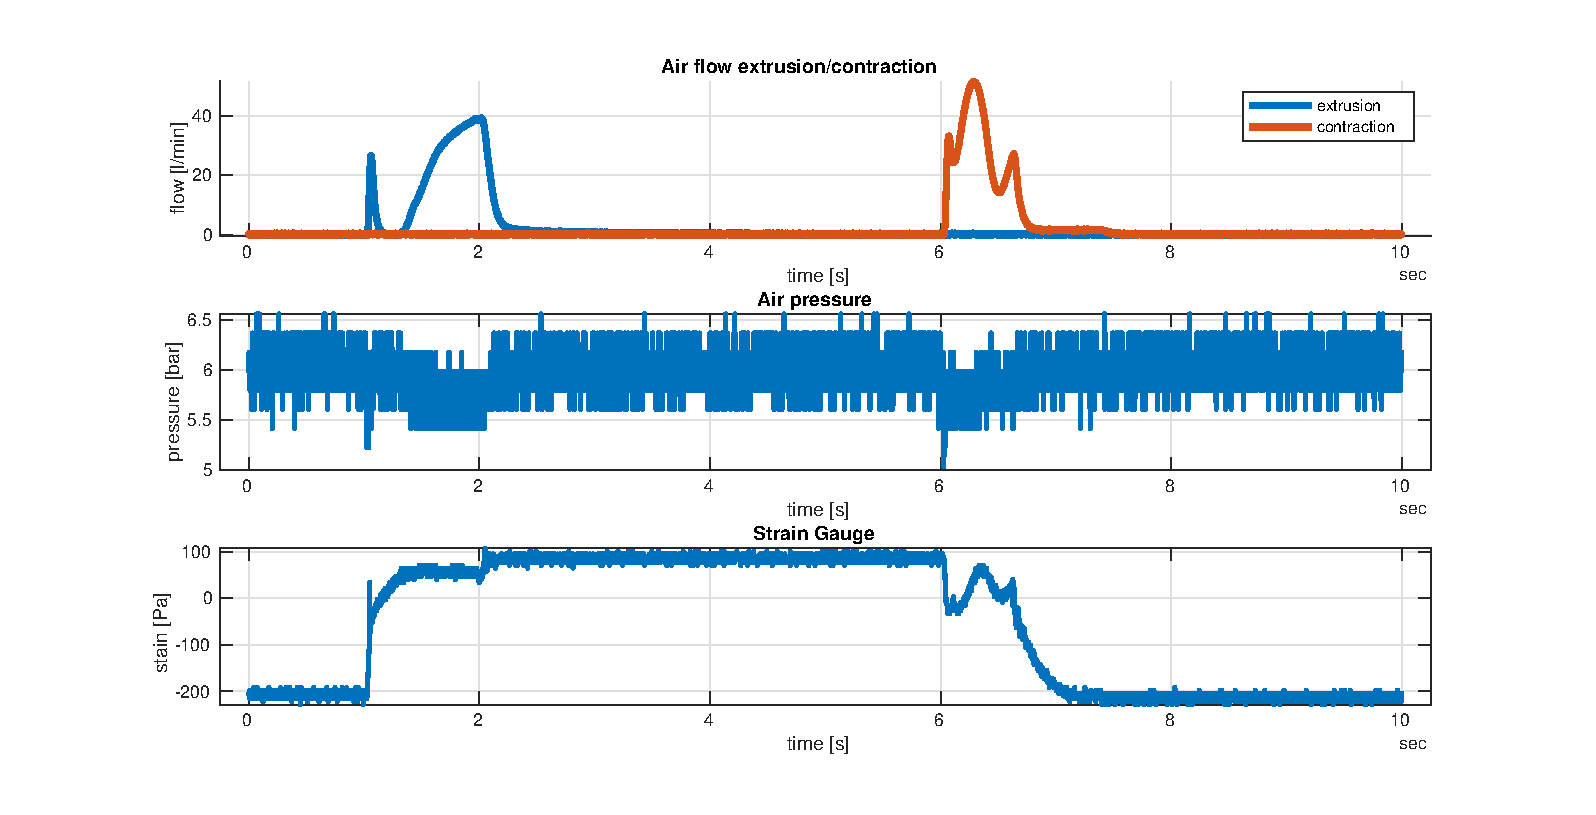
\includegraphics[width=\maxwidth{100.35122930255896em}]{figure_0.eps}
\end{center}
\begin{center}
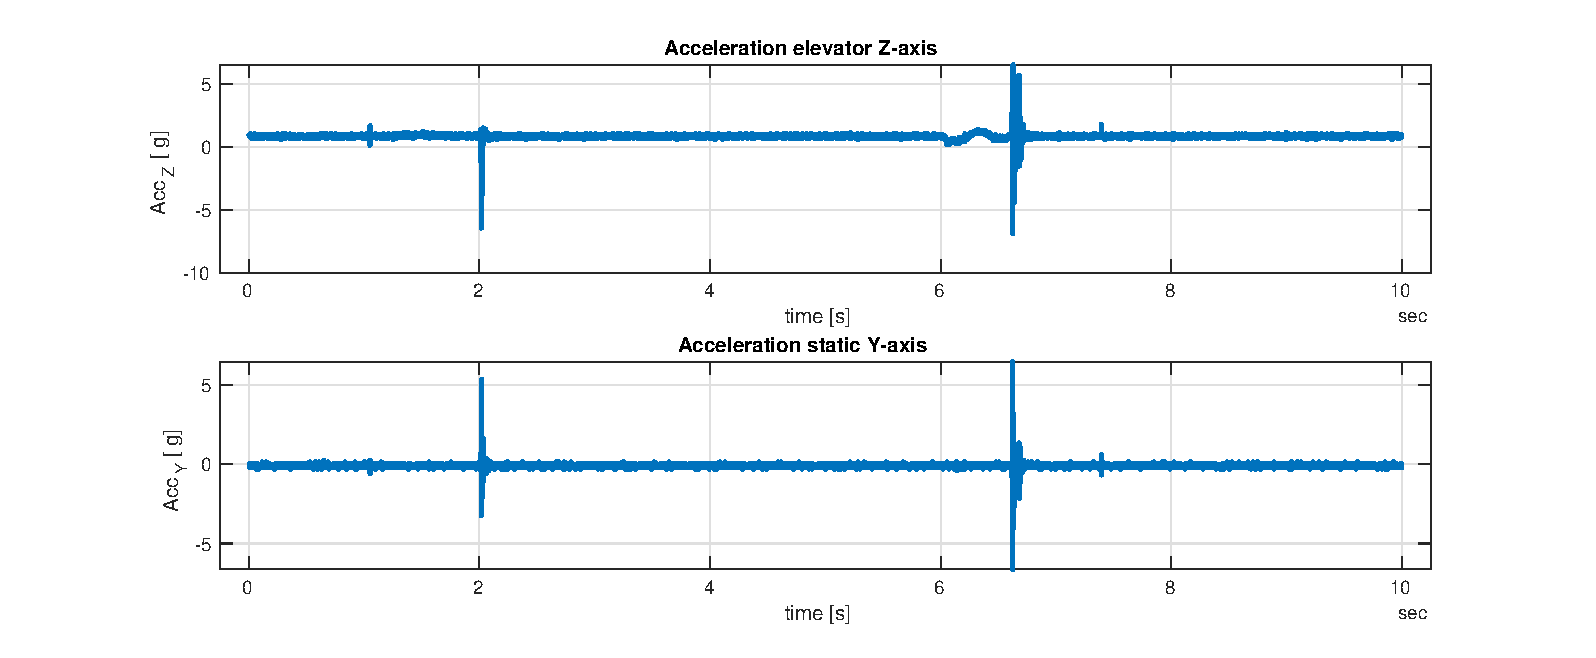
\includegraphics[width=\maxwidth{100.35122930255896em}]{figure_1.eps}
\end{center}
\begin{center}
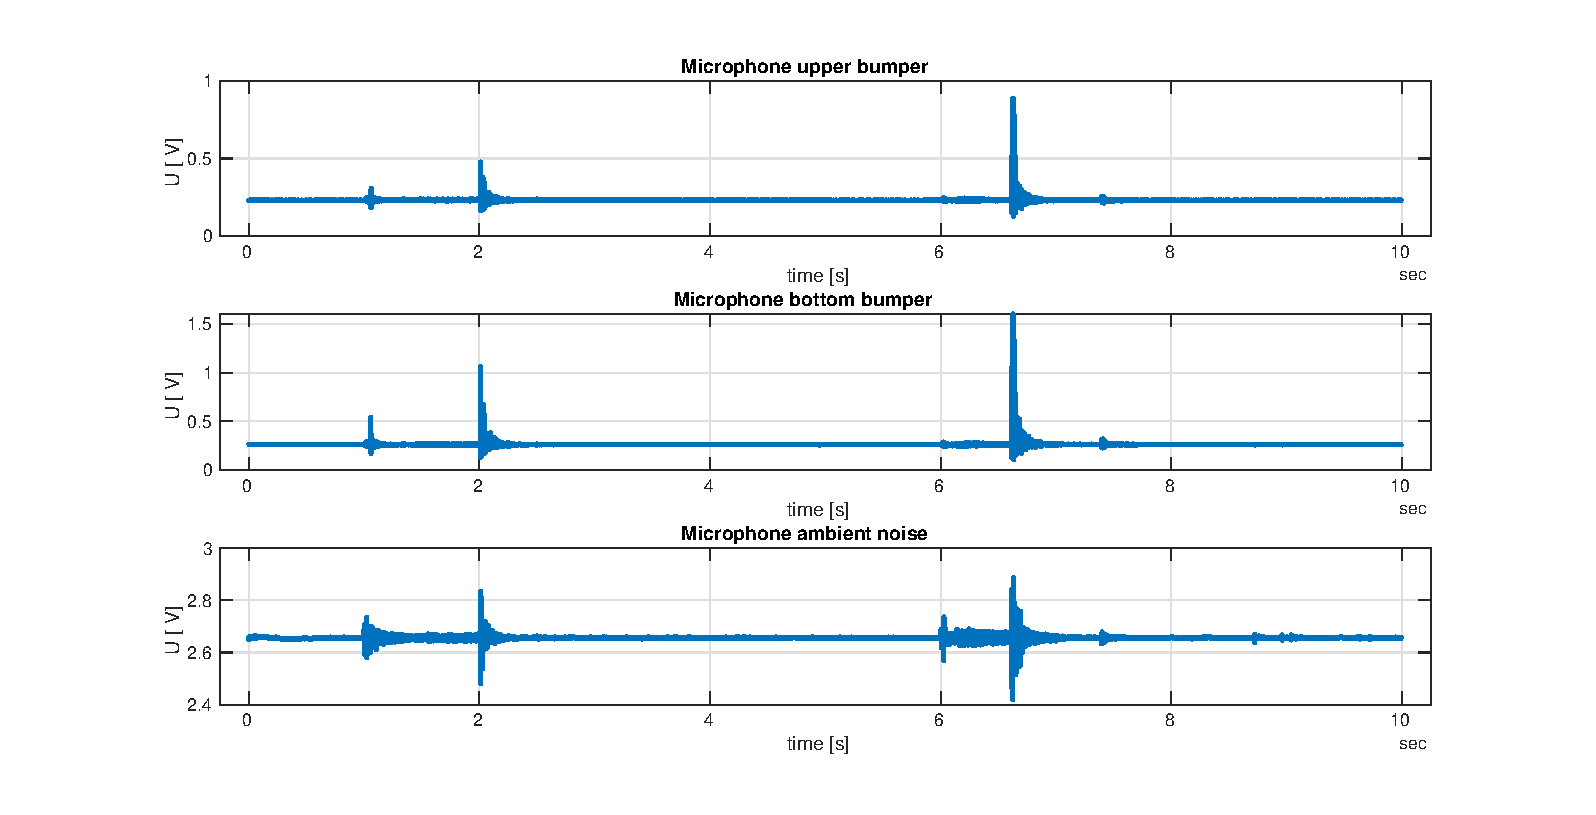
\includegraphics[width=\maxwidth{100.35122930255896em}]{figure_2.eps}
\end{center}
\begin{center}
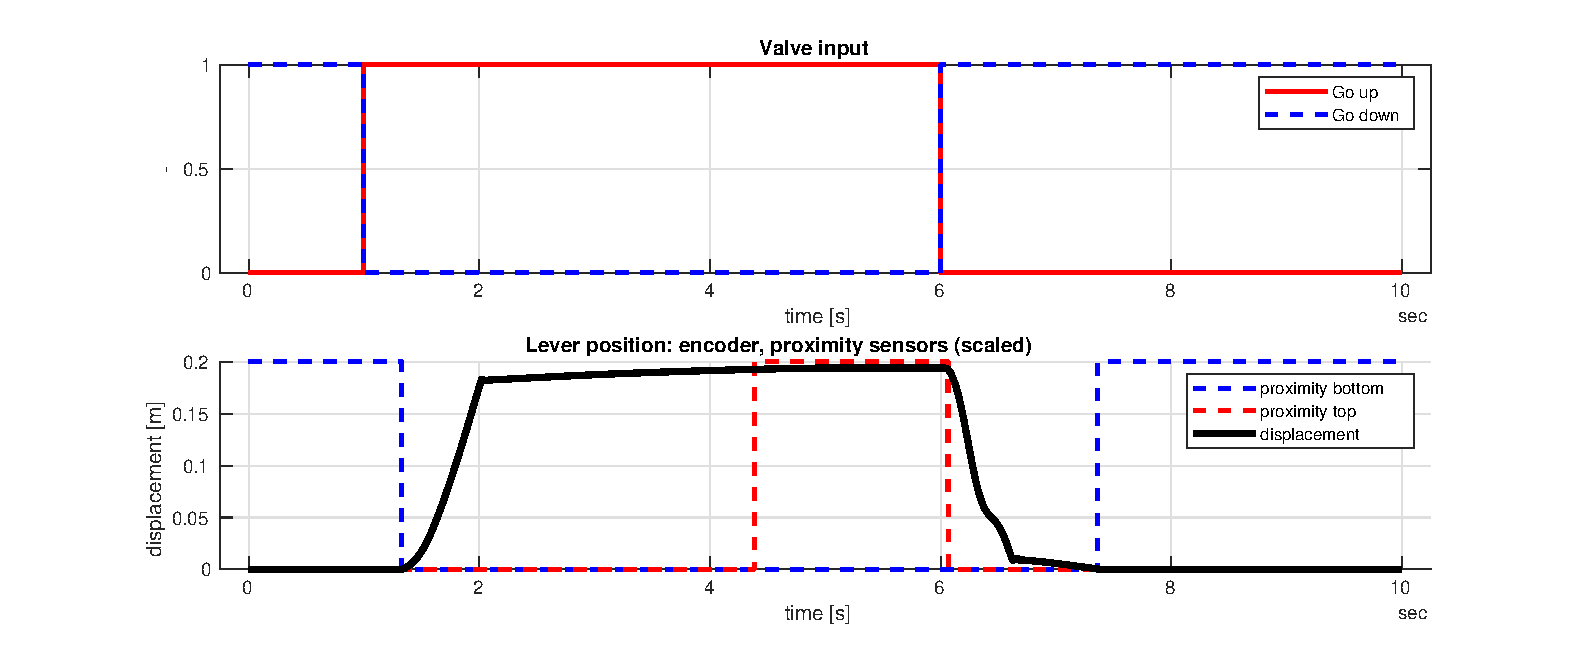
\includegraphics[width=\maxwidth{100.35122930255896em}]{figure_3.eps}
\end{center}

\label{H_50C30838}
\matlabheadingtwo{Raw vs Preprocess}

\begin{par}
\begin{flushleft}
Some signals, such as Encoder, are very accurate. There is no preprocessing needed to apply. Signals noisier (Pressure signal or Strain) has to be preprocessed and applied some noise reduction algorithms. However, during experiments turned out that non preprocessed signals have better performance.  For example, the preprocessed Pressure classification model gives 78\% accuracy; the raw pressure signal gives approximately 82\%.
\end{flushleft}
\end{par}

\begin{par}
\begin{flushleft}
TODO add models
\end{flushleft}
\end{par}


\vspace{1em}

\label{H_EFED6273}
\matlabheading{Encoder}

\begin{par}
\begin{flushleft}
This sensor contain Lever Position. From this position velocity was calculated too. 
\end{flushleft}
\end{par}

\label{H_14C15B00}
\matlabheadingtwo{Extracted features}

\begin{matlabcode}
encoder_cost = 25000;
encoder_suitability = 0.1;
addpath("sensor_encoder/")
features = load("sensor_encoder/LeverPosition_LeverVelocity_stat_features.mat").LeverPosition_LeverVelocity_stat_features;
\end{matlabcode}


\vspace{1em}
\begin{par}
\begin{flushleft}
We can rank features using Kruskall-Wallis analysis of variation to reduce number of features.
\end{flushleft}
\end{par}

\begin{matlabcode}
compute_ranking = 0;
if compute_ranking
    [~,encoder_ranked_features,~] = encoder_features_process(features);
else
    encoder_ranked_features = load("sensor_encoder/encoder_stat_features_ranked.mat").encoder_stat_features_ranked
end
\end{matlabcode}
\begin{matlabtableoutput}
{
\begin{tabular} {|c|c|c|}\hline
\mlcell{ } & \mlcell{Features} & \mlcell{Kruskal-Wallis} \\ \hline
\mlcell{1} & \mlcell{"LeverPosition\_stats/RMS"} & \mlcell{1.0402e+03} \\ \hline
\mlcell{2} & \mlcell{"LeverPosition\_stats/Kurtosis"} & \mlcell{825.0712} \\ \hline
\mlcell{3} & \mlcell{"LeverPosition\_stats/Mean"} & \mlcell{613.0104} \\ \hline
\mlcell{4} & \mlcell{"LeverVelocity\_stats/Mean"} & \mlcell{520.3488} \\ \hline
\mlcell{5} & \mlcell{"LeverPosition\_stats/ImpulseFactor"} & \mlcell{507.9940} \\ \hline
\mlcell{6} & \mlcell{"LeverPosition\_stats/ClearanceFactor"} & \mlcell{478.7457} \\ \hline
\mlcell{7} & \mlcell{"LeverPosition\_stats/Skewness"} & \mlcell{434.7553} \\ \hline
\mlcell{8} & \mlcell{"LeverPosition\_stats/CrestFactor"} & \mlcell{354.7096} \\ \hline
\mlcell{9} & \mlcell{"LeverVelocity\_stats/CrestFactor"} & \mlcell{333.1497} \\ \hline
\mlcell{10} & \mlcell{"LeverVelocity\_stats/SINAD"} & \mlcell{284.7456} \\ \hline
\mlcell{11} & \mlcell{"LeverVelocity\_stats/Kurtosis"} & \mlcell{277.3044} \\ \hline
\mlcell{12} & \mlcell{"LeverPosition\_stats/ShapeFactor"} & \mlcell{258.3271} \\ \hline
\mlcell{13} & \mlcell{"LeverPosition\_stats/THD"} & \mlcell{228.3308} \\ \hline
\mlcell{14} & \mlcell{"LeverVelocity\_stats/RMS"} & \mlcell{214.3044} \\ \hline
\mlcell{15} & \mlcell{"LeverVelocity\_stats/ClearanceFactor"} & \mlcell{204.3625} \\ \hline
\mlcell{16} & \mlcell{"LeverVelocity\_stats/THD"} & \mlcell{198.4401} \\ \hline
\mlcell{17} & \mlcell{"LeverVelocity\_stats/Std"} & \mlcell{186.7020} \\ \hline
\mlcell{18} & \mlcell{"LeverVelocity\_stats/SNR"} & \mlcell{176.0410} \\ \hline
\mlcell{19} & \mlcell{"LeverPosition\_stats/Std"} & \mlcell{165.1620} \\ \hline
\mlcell{20} & \mlcell{"LeverVelocity\_stats/PeakValue"} & \mlcell{158.6114} \\ \hline
\mlcell{21} & \mlcell{"LeverPosition\_stats/PeakValue"} & \mlcell{145.5950} \\ \hline
\mlcell{22} & \mlcell{"LeverVelocity\_stats/ImpulseFactor"} & \mlcell{127.5223} \\ \hline
\mlcell{23} & \mlcell{"LeverVelocity\_stats/Skewness"} & \mlcell{127.1756} \\ \hline
\mlcell{24} & \mlcell{"LeverVelocity\_stats/ShapeFactor"} & \mlcell{115.6315} \\ \hline
\mlcell{25} & \mlcell{"LeverPosition\_stats/SNR"} & \mlcell{113.1321} \\ \hline
\mlcell{26} & \mlcell{"LeverPosition\_stats/SINAD"} & \mlcell{104.6577} \\ 
\hline
\end{tabular}
}
\end{matlabtableoutput}

\begin{par}
\begin{flushleft}
Using only first 5 features \textit{encoder\_static\_feature\_model  }was trained.
\end{flushleft}
\end{par}

\begin{par}
\begin{flushleft}
Reduce extracted features for first five features.
\end{flushleft}
\end{par}

\begin{matlabcode}
first_five_features = encoder_ranked_features.Features(1:5);
reduced_features_with_label = [first_five_features;"Label"];
reduced_features = features(:, reduced_features_with_label);
[train_data, test_data] = split_dataset(reduced_features);
\end{matlabcode}

\label{H_393D5508}
\matlabheadingtwo{Classification model based on encoder signals}

\begin{matlabcode}
[encoder_model, ~] = encoder_FineKNN_train(train_data);
encoder_accuracy = confusion_matrix_plot_handler(encoder_model, test_data);
\end{matlabcode}
\begin{matlaboutput}
Accuracy is 97.25 % 
\end{matlaboutput}
\begin{center}
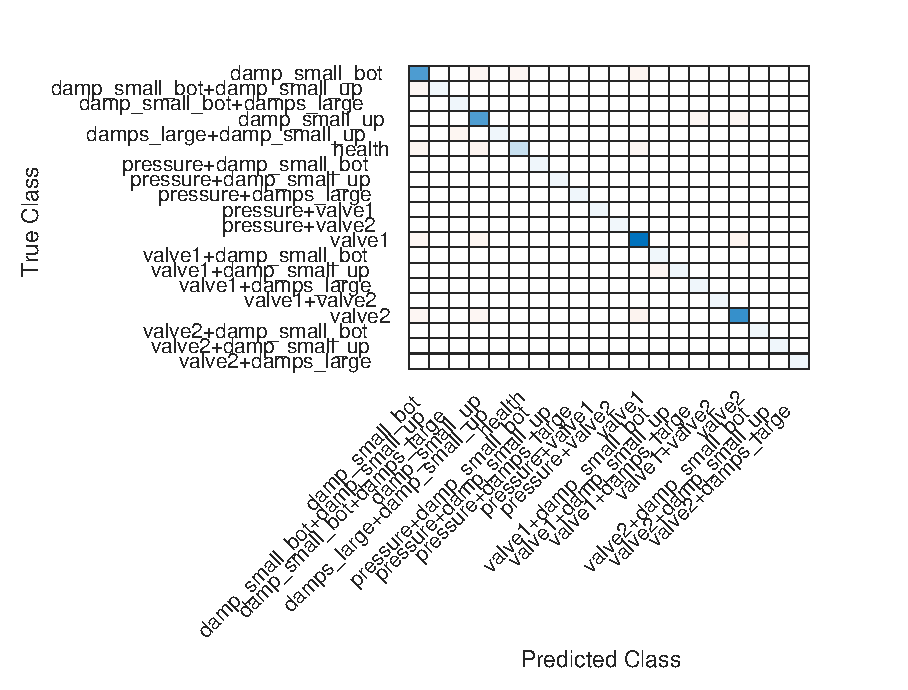
\includegraphics[width=\maxwidth{56.196688409433015em}]{figure_4.eps}
\end{center}

\label{H_7B0AD8F2}
\matlabheadingtwo{Conclusion}

\label{H_6D93AC69}
\begin{par}
\begin{flushleft}
It's possible to achieve 97 \% accuracy, using only the first five ranked statistical features extracted from the system position signal.
\end{flushleft}
\end{par}

\begin{matlabcode}
results_table.("Encoder") = table(encoder_accuracy, encoder_cost, encoder_suitability, 'VariableNames', {'Perfomance', 'Cost', 'Suitability'});
\end{matlabcode}


\label{H_8A224DDB}
\matlabheading{Microphones}

\begin{par}
\begin{flushleft}
There are 3 microphones on stand. 
\end{flushleft}
\end{par}

\begin{enumerate}
\setlength{\itemsep}{-1ex}
   \item{\begin{flushleft} Upper bamper microphone \end{flushleft}}
   \item{\begin{flushleft} Bottom bamper micrphone \end{flushleft}}
   \item{\begin{flushleft} Ambient microphone \end{flushleft}}
\end{enumerate}

\begin{matlabcode}
mics_cost = 500*3;
mics_suitability = 1;
addpath("sensor_mics/")
features = load("sensor_mics/MICsFeaturesAll.mat").MICsFeaturesAll;
if compute_ranking
    [~,mics_ranked_features,~] = mics_features_process(features)
else
    mics_ranked_features = load("sensor_mics/mics_ranked_features.mat").mics_ranked_features
end
\end{matlabcode}
\begin{matlabtableoutput}
{
\begin{tabular} {|c|c|c|}\hline
\mlcell{ } & \mlcell{Features} & \mlcell{Kruskal-Wallis} \\ \hline
\mlcell{1} & \mlcell{"MIC\_uBumper\_stats/SNR"} & \mlcell{1.4156e+03} \\ \hline
\mlcell{2} & \mlcell{"MIC\_Ambient\_ps\_spec/PeakAmp3"} & \mlcell{783.1897} \\ \hline
\mlcell{3} & \mlcell{"MIC\_Ambient\_stats/RMS"} & \mlcell{697.9581} \\ \hline
\mlcell{4} & \mlcell{"MIC\_bBumper\_ps\_spec/PeakFreq4"} & \mlcell{691.1838} \\ \hline
\mlcell{5} & \mlcell{"MIC\_uBumper\_ps\_spec/PeakAmp1"} & \mlcell{677.6992} \\ \hline
\mlcell{6} & \mlcell{"MIC\_uBumper\_stats/SINAD"} & \mlcell{637.4455} \\ \hline
\mlcell{7} & \mlcell{"MIC\_Ambient\_stats/Mean"} & \mlcell{586.2918} \\ \hline
\mlcell{8} & \mlcell{"MIC\_bBumper\_ps\_spec/PeakFreq2"} & \mlcell{573.6578} \\ \hline
\mlcell{9} & \mlcell{"MIC\_Ambient\_ps\_spec/BandPower"} & \mlcell{566.5475} \\ \hline
\mlcell{10} & \mlcell{"MIC\_uBumper\_ps\_spec/BandPower"} & \mlcell{521.9659} \\ \hline
\mlcell{11} & \mlcell{"MIC\_Ambient\_ps\_spec/PeakAmp8"} & \mlcell{514.1117} \\ \hline
\mlcell{12} & \mlcell{"MIC\_Ambient\_ps\_spec/PeakAmp1"} & \mlcell{504.3916} \\ \hline
\mlcell{13} & \mlcell{"MIC\_bBumper\_ps\_spec/PeakFreq1"} & \mlcell{488.1185} \\ \hline
\mlcell{14} & \mlcell{"MIC\_uBumper\_stats/RMS"} & \mlcell{470.3004} \\ \hline
\mlcell{15} & \mlcell{"MIC\_uBumper\_stats/Mean"} & \mlcell{446.3744} \\ \hline
\mlcell{16} & \mlcell{"MIC\_Ambient\_ps\_spec/PeakAmp4"} & \mlcell{439.4747} \\ \hline
\mlcell{17} & \mlcell{"MIC\_uBumper\_ps\_spec/PeakAmp3"} & \mlcell{434.5301} \\ \hline
\mlcell{18} & \mlcell{"MIC\_Ambient\_ps\_spec/PeakAmp2"} & \mlcell{416.4112} \\ \hline
\mlcell{19} & \mlcell{"MIC\_bBumper\_ps\_spec/PeakAmp5"} & \mlcell{408.1541} \\ \hline
\mlcell{20} & \mlcell{"MIC\_Ambient\_ps\_spec/PeakAmp5"} & \mlcell{397.7929} \\ \hline
\mlcell{21} & \mlcell{"MIC\_bBumper\_stats/THD"} & \mlcell{375.6265} \\ \hline
\mlcell{22} & \mlcell{"MIC\_bBumper\_ps\_spec/PeakAmp6"} & \mlcell{373.1111} \\ \hline
\mlcell{23} & \mlcell{"MIC\_Ambient\_ps\_spec/PeakAmp6"} & \mlcell{371.4687} \\ \hline
\mlcell{24} & \mlcell{"MIC\_Ambient\_ps\_spec/PeakAmp10"} & \mlcell{347.7271} \\ \hline
\mlcell{25} & \mlcell{"MIC\_bBumper\_stats/Mean"} & \mlcell{346.9966} \\ \hline
\mlcell{26} & \mlcell{"MIC\_uBumper\_stats/ShapeFactor"} & \mlcell{343.1625} \\ \hline
\mlcell{27} & \mlcell{"MIC\_Ambient\_ps\_spec/PeakAmp9"} & \mlcell{342.0259} \\ \hline
\mlcell{28} & \mlcell{"MIC\_bBumper\_ps\_spec/PeakAmp4"} & \mlcell{334.6862} \\ \hline
\mlcell{29} & \mlcell{"MIC\_Ambient\_ps\_spec/PeakAmp7"} & \mlcell{322.8021} \\ \hline
\mlcell{30} & \mlcell{"MIC\_bBumper\_stats/RMS"} & \mlcell{319.8055} \\ \hline
\mlcell{31} & \mlcell{"MIC\_uBumper\_ps\_spec/PeakAmp8"} & \mlcell{315.9739} \\ \hline
\mlcell{32} & \mlcell{"MIC\_uBumper\_ps\_spec/PeakFreq9"} & \mlcell{315.7096} \\ \hline
\mlcell{33} & \mlcell{"MIC\_uBumper\_ps\_spec/PeakAmp4"} & \mlcell{304.1032} \\ \hline
\mlcell{34} & \mlcell{"MIC\_bBumper\_ps\_spec/PeakAmp7"} & \mlcell{296.5131} \\ \hline
\mlcell{35} & \mlcell{"MIC\_bBumper\_ps\_spec/BandPower"} & \mlcell{290.5723} \\ \hline
\mlcell{36} & \mlcell{"MIC\_bBumper\_stats/SINAD"} & \mlcell{286.9970} \\ \hline
\mlcell{37} & \mlcell{"MIC\_bBumper\_stats/SNR"} & \mlcell{281.5116} \\ \hline
\mlcell{38} & \mlcell{"MIC\_uBumper\_ps\_spec/PeakAmp10"} & \mlcell{280.8211} \\ \hline
\mlcell{39} & \mlcell{"MIC\_uBumper\_stats/Kurtosis"} & \mlcell{270.0994} \\ \hline
\mlcell{40} & \mlcell{"MIC\_bBumper\_ps\_spec/PeakAmp3"} & \mlcell{267.3615} \\ \hline
\mlcell{41} & \mlcell{"MIC\_bBumper\_stats/ShapeFactor"} & \mlcell{255.6624} \\ \hline
\mlcell{42} & \mlcell{"MIC\_uBumper\_ps\_spec/PeakFreq2"} & \mlcell{254.0944} \\ \hline
\mlcell{43} & \mlcell{"MIC\_bBumper\_ps\_spec/PeakAmp10"} & \mlcell{247.9684} \\ \hline
\mlcell{44} & \mlcell{"MIC\_uBumper\_ps\_spec/PeakAmp6"} & \mlcell{238.3955} \\ \hline
\mlcell{45} & \mlcell{"MIC\_Ambient\_stats/Kurtosis"} & \mlcell{236.0343} \\ \hline
\mlcell{46} & \mlcell{"MIC\_bBumper\_ps\_spec/PeakAmp8"} & \mlcell{230.5929} \\ \hline
\mlcell{47} & \mlcell{"MIC\_uBumper\_stats/Skewness"} & \mlcell{229.4500} \\ \hline
\mlcell{48} & \mlcell{"MIC\_bBumper\_ps\_spec/PeakAmp9"} & \mlcell{224.6076} \\ \hline
\mlcell{49} & \mlcell{"MIC\_uBumper\_ps\_spec/PeakAmp5"} & \mlcell{220.7581} \\ \hline
\mlcell{50} & \mlcell{"MIC\_bBumper\_ps\_spec/PeakFreq3"} & \mlcell{218.5680} \\ \hline
\mlcell{51} & \mlcell{"MIC\_uBumper\_stats/Std"} & \mlcell{217.0325} \\ \hline
\mlcell{52} & \mlcell{"MIC\_bBumper\_stats/Kurtosis"} & \mlcell{214.7843} \\ \hline
\mlcell{53} & \mlcell{"MIC\_bBumper\_ps\_spec/PeakFreq5"} & \mlcell{214.4877} \\ \hline
\mlcell{54} & \mlcell{"MIC\_Ambient\_stats/THD"} & \mlcell{214.0941} \\ \hline
\mlcell{55} & \mlcell{"MIC\_Ambient\_stats/ShapeFactor"} & \mlcell{213.0586} \\ \hline
\mlcell{56} & \mlcell{"MIC\_bBumper\_ps\_spec/PeakAmp1"} & \mlcell{211.6635} \\ \hline
\mlcell{57} & \mlcell{"MIC\_bBumper\_ps\_spec/PeakAmp2"} & \mlcell{203.5507} \\ \hline
\mlcell{58} & \mlcell{"MIC\_uBumper\_ps\_spec/PeakAmp9"} & \mlcell{192.9091} \\ \hline
\mlcell{59} & \mlcell{"MIC\_bBumper\_stats/Std"} & \mlcell{184.6081} \\ \hline
\mlcell{60} & \mlcell{"MIC\_Ambient\_stats/SINAD"} & \mlcell{182.7846} \\ \hline
\mlcell{61} & \mlcell{"MIC\_Ambient\_stats/SNR"} & \mlcell{180.1587} \\ \hline
\mlcell{62} & \mlcell{"MIC\_uBumper\_ps\_spec/PeakAmp2"} & \mlcell{179.9498} \\ \hline
\mlcell{63} & \mlcell{"MIC\_uBumper\_ps\_spec/PeakFreq10"} & \mlcell{179.9065} \\ \hline
\mlcell{64} & \mlcell{"MIC\_bBumper\_stats/Skewness"} & \mlcell{179.5166} \\ \hline
\mlcell{65} & \mlcell{"MIC\_bBumper\_ps\_spec/PeakFreq6"} & \mlcell{177.5985} \\ \hline
\mlcell{66} & \mlcell{"MIC\_uBumper\_ps\_spec/PeakFreq7"} & \mlcell{176.0634} \\ \hline
\mlcell{67} & \mlcell{"MIC\_uBumper\_ps\_spec/PeakFreq1"} & \mlcell{170.7543} \\ \hline
\mlcell{68} & \mlcell{"MIC\_Ambient\_stats/Skewness"} & \mlcell{170.1383} \\ \hline
\mlcell{69} & \mlcell{"MIC\_uBumper\_ps\_spec/PeakAmp7"} & \mlcell{168.8676} \\ \hline
\mlcell{70} & \mlcell{"MIC\_uBumper\_ps\_spec/PeakFreq5"} & \mlcell{160.2663} \\ \hline
\mlcell{71} & \mlcell{"MIC\_uBumper\_ps\_spec/PeakFreq8"} & \mlcell{154.8746} \\ \hline
\mlcell{72} & \mlcell{"MIC\_uBumper\_stats/PeakValue"} & \mlcell{154.2331} \\ \hline
\mlcell{73} & \mlcell{"MIC\_uBumper\_stats/ClearanceFactor"} & \mlcell{151.6394} \\ \hline
\mlcell{74} & \mlcell{"MIC\_uBumper\_stats/ImpulseFactor"} & \mlcell{149.5290} \\ \hline
\mlcell{75} & \mlcell{"MIC\_uBumper\_stats/CrestFactor"} & \mlcell{147.1777} \\ \hline
\mlcell{76} & \mlcell{"MIC\_Ambient\_stats/Std"} & \mlcell{136.4742} \\ \hline
\mlcell{77} & \mlcell{"MIC\_Ambient\_stats/PeakValue"} & \mlcell{124.6259} \\ \hline
\mlcell{78} & \mlcell{"MIC\_bBumper\_ps\_spec/PeakFreq10"} & \mlcell{119.2369} \\ \hline
\mlcell{79} & \mlcell{"MIC\_bBumper\_stats/CrestFactor"} & \mlcell{113.2928} \\ \hline
\mlcell{80} & \mlcell{"MIC\_Ambient\_stats/CrestFactor"} & \mlcell{110.5332} \\ \hline
\mlcell{81} & \mlcell{"MIC\_bBumper\_stats/ImpulseFactor"} & \mlcell{109.3978} \\ \hline
\mlcell{82} & \mlcell{"MIC\_Ambient\_stats/ClearanceFactor"} & \mlcell{108.0850} \\ \hline
\mlcell{83} & \mlcell{"MIC\_bBumper\_stats/ClearanceFactor"} & \mlcell{106.8416} \\ \hline
\mlcell{84} & \mlcell{"MIC\_Ambient\_stats/ImpulseFactor"} & \mlcell{105.7583} \\ \hline
\mlcell{85} & \mlcell{"MIC\_bBumper\_ps\_spec/PeakFreq8"} & \mlcell{102.2267} \\ \hline
\mlcell{86} & \mlcell{"MIC\_bBumper\_stats/PeakValue"} & \mlcell{100.1652} \\ \hline
\mlcell{87} & \mlcell{"MIC\_uBumper\_ps\_spec/PeakFreq3"} & \mlcell{91.1485} \\ \hline
\mlcell{88} & \mlcell{"MIC\_bBumper\_ps\_spec/PeakFreq7"} & \mlcell{84.1486} \\ \hline
\mlcell{89} & \mlcell{"MIC\_bBumper\_ps\_spec/PeakFreq9"} & \mlcell{68.8097} \\ \hline
\mlcell{90} & \mlcell{"MIC\_uBumper\_ps\_spec/PeakFreq6"} & \mlcell{59.1941} \\ \hline
\mlcell{91} & \mlcell{"MIC\_Ambient\_ps\_spec/PeakFreq9"} & \mlcell{24.2495} \\ \hline
\mlcell{92} & \mlcell{"MIC\_Ambient\_ps\_spec/PeakFreq2"} & \mlcell{16.3744} \\ \hline
\mlcell{93} & \mlcell{"MIC\_Ambient\_ps\_spec/PeakFreq10"} & \mlcell{10.4624} \\ \hline
\mlcell{94} & \mlcell{"MIC\_Ambient\_ps\_spec/PeakFreq3"} & \mlcell{8.1067} \\ \hline
\mlcell{95} & \mlcell{"MIC\_uBumper\_ps\_spec/PeakFreq4"} & \mlcell{7.7865} \\ \hline
\mlcell{96} & \mlcell{"MIC\_Ambient\_ps\_spec/PeakFreq4"} & \mlcell{6.3615} \\ \hline
\mlcell{97} & \mlcell{"MIC\_Ambient\_ps\_spec/PeakFreq8"} & \mlcell{5.1293} \\ \hline
\mlcell{98} & \mlcell{"MIC\_Ambient\_ps\_spec/PeakFreq6"} & \mlcell{4.2943} \\ \hline
\mlcell{99} & \mlcell{"MIC\_Ambient\_ps\_spec/PeakFreq7"} & \mlcell{3.8876} \\ \hline
\mlcell{100} & \mlcell{"MIC\_Ambient\_ps\_spec/PeakFreq5"} & \mlcell{3.8352} \\ 
\hline
\end{tabular}
}
\end{matlabtableoutput}
\begin{matlabcode}
first_five_features = mics_ranked_features.Features(1:5)
\end{matlabcode}
\begin{matlaboutput}
first_five_features = 5x1 string    
"MIC_uBumper_stats/SNR"        
"MIC_Ambient_ps_spec/PeakAmp3" 
"MIC_Ambient_stats/RMS"        
"MIC_bBumper_ps_spec/PeakFreq4"
"MIC_uBumper_ps_spec/PeakAmp1" 

\end{matlaboutput}
\begin{matlabcode}
reduced_features_with_label = [first_five_features;"Label"];
reduced_features = features(:, reduced_features_with_label);
[train_data, test_data] = split_dataset(reduced_features);

[mics_model, ~ ] = mics_BaggedTrees_train(train_data);
mics_accuracy = confusion_matrix_plot_handler(mics_model, test_data);
\end{matlabcode}
\begin{matlaboutput}
Accuracy is 94.77 % 
\end{matlaboutput}
\begin{center}
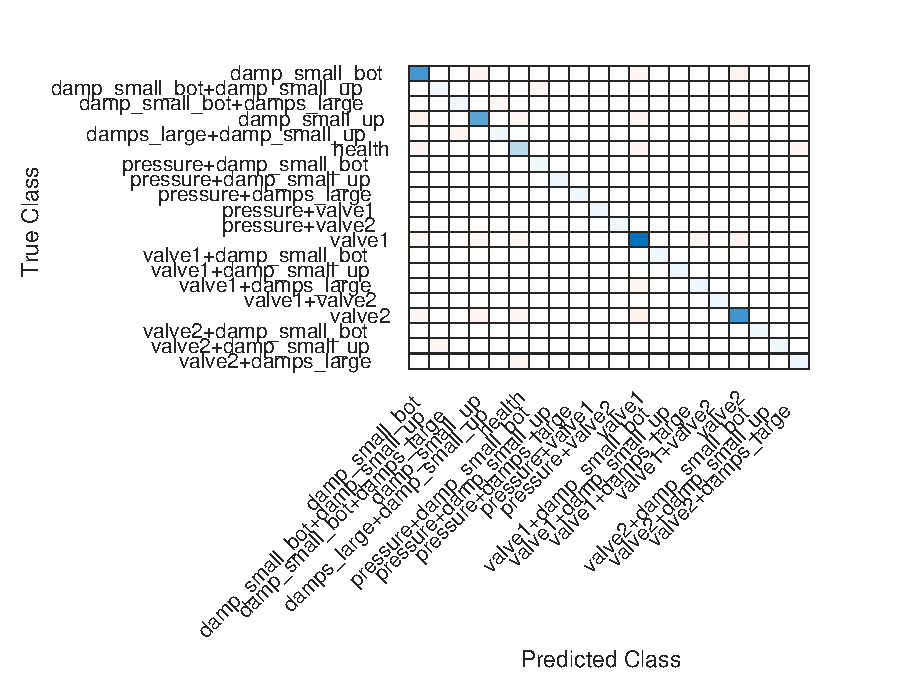
\includegraphics[width=\maxwidth{56.196688409433015em}]{figure_5.eps}
\end{center}

\label{H_5E913988}
\matlabheadingtwo{Conclusion}

\begin{matlabcode}
results_table.("Mics") = table(mics_accuracy, mics_cost, mics_suitability, 'VariableNames', {'Perfomance', 'Cost', 'Suitability'});
\end{matlabcode}


\label{H_D4E209E2}
\matlabheading{Flow Sensors}

\begin{par}
\begin{flushleft}
There are two signals measured:
\end{flushleft}
\end{par}

\begin{enumerate}
\setlength{\itemsep}{-1ex}
   \item{\begin{flushleft} Flow Exrusion \end{flushleft}}
   \item{\begin{flushleft} Flow Contraction \end{flushleft}}
\end{enumerate}

\begin{matlabcode}
flow_cost = 12000;
flow_suitability = 0.5;

addpath("sensor_flow/");
features = load("sensor_flow/FlowsFeaturesAll.mat").FlowsFeaturesAll
\end{matlabcode}

\begin{matlabcode}
if compute_ranking
    [~,flow_ranked_features,~] = flow_features_process(features)
else
    flow_ranked_features = load("sensor_flow/flow_ranked_features.mat").flow_ranked_features
end
\end{matlabcode}
\begin{matlabtableoutput}
{
\begin{tabular} {|c|c|c|}\hline
\mlcell{ } & \mlcell{Features} & \mlcell{Kruskal-Wallis} \\ \hline
\mlcell{1} & \mlcell{"FlowContraction\_ps\_spec/PeakAmp1"} & \mlcell{1.4815e+03} \\ \hline
\mlcell{2} & \mlcell{"FlowContraction\_stats/CrestFactor"} & \mlcell{967.6028} \\ \hline
\mlcell{3} & \mlcell{"FlowContraction\_ps\_spec/PeakAmp3"} & \mlcell{865.7571} \\ \hline
\mlcell{4} & \mlcell{"FlowContraction\_stats/Mean"} & \mlcell{567.6620} \\ \hline
\mlcell{5} & \mlcell{"FlowExtrusion\_stats/SNR"} & \mlcell{558.1070} \\ \hline
\mlcell{6} & \mlcell{"FlowContraction\_ps\_spec/PeakAmp4"} & \mlcell{460.0924} \\ \hline
\mlcell{7} & \mlcell{"FlowContraction\_stats/Kurtosis"} & \mlcell{424.0319} \\ \hline
\mlcell{8} & \mlcell{"FlowExtrusion\_stats/SINAD"} & \mlcell{416.9781} \\ \hline
\mlcell{9} & \mlcell{"FlowExtrusion\_stats/CrestFactor"} & \mlcell{379.8486} \\ \hline
\mlcell{10} & \mlcell{"FlowContraction\_ps\_spec/PeakFreq3"} & \mlcell{317.7894} \\ \hline
\mlcell{11} & \mlcell{"FlowContraction\_ps\_spec/PeakAmp5"} & \mlcell{279.8224} \\ \hline
\mlcell{12} & \mlcell{"FlowExtrusion\_stats/PeakValue"} & \mlcell{247.6351} \\ \hline
\mlcell{13} & \mlcell{"FlowExtrusion\_ps\_spec/PeakFreq2"} & \mlcell{241.1545} \\ \hline
\mlcell{14} & \mlcell{"FlowContraction\_stats/THD"} & \mlcell{239.3326} \\ \hline
\mlcell{15} & \mlcell{"FlowExtrusion\_stats/Kurtosis"} & \mlcell{233.3454} \\ \hline
\mlcell{16} & \mlcell{"FlowContraction\_ps\_spec/PeakFreq2"} & \mlcell{220.8141} \\ \hline
\mlcell{17} & \mlcell{"FlowContraction\_stats/Skewness"} & \mlcell{210.0841} \\ \hline
\mlcell{18} & \mlcell{"FlowContraction\_ps\_spec/BandPower"} & \mlcell{199.0419} \\ \hline
\mlcell{19} & \mlcell{"FlowExtrusion\_stats/ShapeFactor"} & \mlcell{190.3549} \\ \hline
\mlcell{20} & \mlcell{"FlowExtrusion\_ps\_spec/PeakFreq3"} & \mlcell{189.2356} \\ \hline
\mlcell{21} & \mlcell{"FlowExtrusion\_stats/ImpulseFactor"} & \mlcell{183.7506} \\ \hline
\mlcell{22} & \mlcell{"FlowExtrusion\_stats/Mean"} & \mlcell{176.6569} \\ \hline
\mlcell{23} & \mlcell{"FlowContraction\_ps\_spec/PeakFreq5"} & \mlcell{172.1256} \\ \hline
\mlcell{24} & \mlcell{"FlowExtrusion\_stats/Std"} & \mlcell{167.9328} \\ \hline
\mlcell{25} & \mlcell{"FlowExtrusion\_stats/RMS"} & \mlcell{158.3523} \\ \hline
\mlcell{26} & \mlcell{"FlowExtrusion\_ps\_spec/PeakFreq5"} & \mlcell{153.4057} \\ \hline
\mlcell{27} & \mlcell{"FlowExtrusion\_ps\_spec/BandPower"} & \mlcell{151.1453} \\ \hline
\mlcell{28} & \mlcell{"FlowContraction\_stats/ClearanceFactor"} & \mlcell{145.5279} \\ \hline
\mlcell{29} & \mlcell{"FlowExtrusion\_ps\_spec/PeakFreq4"} & \mlcell{145.3355} \\ \hline
\mlcell{30} & \mlcell{"FlowContraction\_ps\_spec/PeakAmp2"} & \mlcell{143.3397} \\ \hline
\mlcell{31} & \mlcell{"FlowExtrusion\_stats/ClearanceFactor"} & \mlcell{143.0809} \\ \hline
\mlcell{32} & \mlcell{"FlowExtrusion\_ps\_spec/PeakAmp5"} & \mlcell{140.8227} \\ \hline
\mlcell{33} & \mlcell{"FlowContraction\_stats/Std"} & \mlcell{133.5302} \\ \hline
\mlcell{34} & \mlcell{"FlowContraction\_stats/RMS"} & \mlcell{128.5736} \\ \hline
\mlcell{35} & \mlcell{"FlowContraction\_ps\_spec/PeakFreq4"} & \mlcell{127.6140} \\ \hline
\mlcell{36} & \mlcell{"FlowExtrusion\_stats/Skewness"} & \mlcell{121.5375} \\ \hline
\mlcell{37} & \mlcell{"FlowContraction\_stats/ImpulseFactor"} & \mlcell{112.0391} \\ \hline
\mlcell{38} & \mlcell{"FlowContraction\_stats/ShapeFactor"} & \mlcell{106.8762} \\ \hline
\mlcell{39} & \mlcell{"FlowExtrusion\_ps\_spec/PeakAmp2"} & \mlcell{105.6735} \\ \hline
\mlcell{40} & \mlcell{"FlowExtrusion\_ps\_spec/PeakAmp3"} & \mlcell{101.9201} \\ \hline
\mlcell{41} & \mlcell{"FlowContraction\_stats/PeakValue"} & \mlcell{98.8923} \\ \hline
\mlcell{42} & \mlcell{"FlowExtrusion\_ps\_spec/PeakAmp4"} & \mlcell{94.4188} \\ \hline
\mlcell{43} & \mlcell{"FlowContraction\_stats/SINAD"} & \mlcell{93.1361} \\ \hline
\mlcell{44} & \mlcell{"FlowExtrusion\_ps\_spec/PeakAmp1"} & \mlcell{85.0454} \\ \hline
\mlcell{45} & \mlcell{"FlowContraction\_stats/SNR"} & \mlcell{76.6229} \\ \hline
\mlcell{46} & \mlcell{"FlowContraction\_ps\_spec/PeakFreq1"} & \mlcell{1.3206} \\ \hline
\mlcell{47} & \mlcell{"FlowExtrusion\_ps\_spec/PeakFreq1"} & \mlcell{1.2925} \\ \hline
\mlcell{48} & \mlcell{"FlowExtrusion\_stats/THD"} & \mlcell{0} \\ 
\hline
\end{tabular}
}
\end{matlabtableoutput}

\begin{par}
\begin{flushleft}
We will use only Flow Contraction signal:
\end{flushleft}
\end{par}

\begin{matlabcode}
reduced_features = [flow_ranked_features.Features(1:4); flow_ranked_features.Features(6)]
\end{matlabcode}
\begin{matlaboutput}
reduced_features = 5x1 string    
"FlowContraction_ps_spec/Pea…  
"FlowContraction_stats/Crest…  
"FlowContraction_ps_spec/Pea…  
"FlowContraction_stats/Mean"   
"FlowContraction_ps_spec/Pea…  

\end{matlaboutput}
\begin{matlabcode}
reduced_features_with_label = [reduced_features;"Label"];
reduced_features = features(:, reduced_features_with_label);
[train_data, test_data] = split_dataset(reduced_features);

[flow_model, ~ ] = train_flow_KNN(train_data);

flow_accuracy = confusion_matrix_plot_handler(flow_model, test_data);
\end{matlabcode}
\begin{matlaboutput}
Accuracy is 97.04 % 
\end{matlaboutput}
\begin{center}
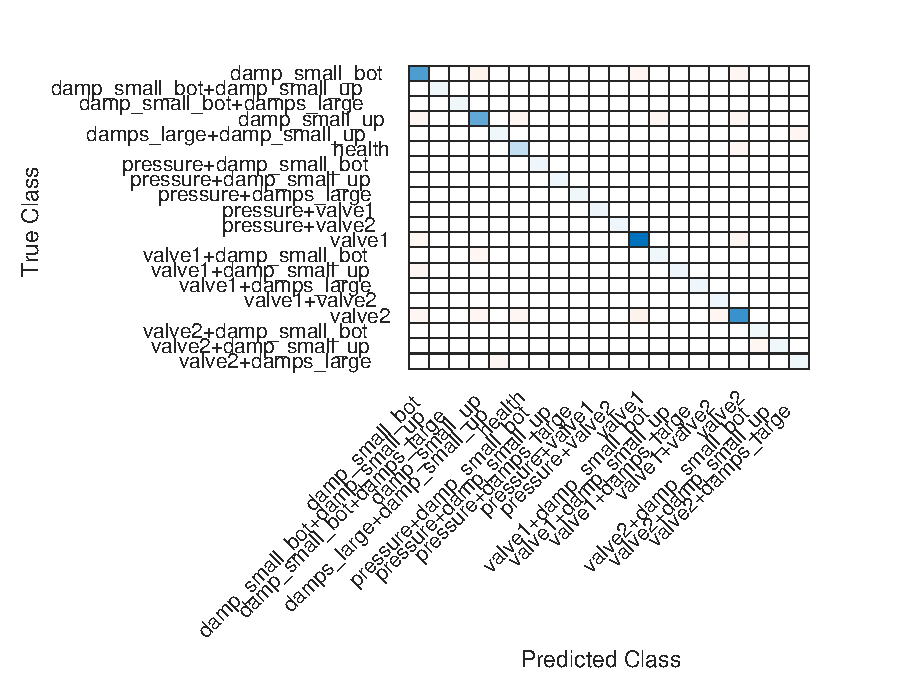
\includegraphics[width=\maxwidth{56.196688409433015em}]{figure_6.eps}
\end{center}

\label{H_911122FE}
\matlabheadingtwo{Conclusion}

\begin{matlabcode}
results_table.("Flow") = table(flow_accuracy, flow_cost, flow_suitability, 'VariableNames', {'Perfomance', 'Cost', 'Suitability'});
\end{matlabcode}


\label{H_F6FCF01A}
\matlabheading{Accelerometer}

\begin{par}
\begin{flushleft}
There are two accelerometer sensors. Each sensor contains two signals in a perpendicular direction. 
\end{flushleft}
\end{par}

\begin{par}
\begin{flushleft}
One sensor is placed on the movable part of the stand device. The second is on the statical part of the stand device.
\end{flushleft}
\end{par}

\begin{matlabcode}
acc_cost = 3500*2;
acc_suitability = 0.5;

addpath("sensor_acc/");
features = load("sensor_acc/AccAllFeatures.mat").AccAllFeatures;
if compute_ranking
    [~,acc_ranked_features,~] = acc_features_process(features)
else
    acc_ranked_features = load("sensor_acc/acc_ranked_features.mat").acc_ranked_features
end
\end{matlabcode}
\begin{matlabtableoutput}
{
\begin{tabular} {|c|c|c|}\hline
\mlcell{ } & \mlcell{Features} & \mlcell{Kruskal-Wallis} \\ \hline
\mlcell{1} & \mlcell{"AccelerometerStatic\_axisY\_stats/ShapeFactor"} & \mlcell{1.0281e+03} \\ \hline
\mlcell{2} & \mlcell{"AccelerometerStatic\_axisZ\_ps\_spec/PeakAmp3"} & \mlcell{576.9968} \\ \hline
\mlcell{3} & \mlcell{"AccelerometerStatic\_axisY\_stats/RMS"} & \mlcell{474.6077} \\ \hline
\mlcell{4} & \mlcell{"AccelerometerStatic\_axisZ\_ps\_spec/PeakAmp10"} & \mlcell{391.5933} \\ \hline
\mlcell{5} & \mlcell{"AccelerometerMoving\_axisZ\_stats/Skewness"} & \mlcell{366.2596} \\ \hline
\mlcell{6} & \mlcell{"AccelerometerStatic\_axisZ\_ps\_spec/PeakAmp4"} & \mlcell{339.0816} \\ \hline
\mlcell{7} & \mlcell{"AccelerometerStatic\_axisZ\_ps\_spec/PeakAmp5"} & \mlcell{319.6353} \\ \hline
\mlcell{8} & \mlcell{"AccelerometerStatic\_axisZ\_ps\_spec/PeakAmp1"} & \mlcell{318.3201} \\ \hline
\mlcell{9} & \mlcell{"AccelerometerStatic\_axisY\_stats/Std"} & \mlcell{295.9981} \\ \hline
\mlcell{10} & \mlcell{"AccelerometerStatic\_axisY\_ps\_spec/BandPower"} & \mlcell{286.3249} \\ \hline
\mlcell{11} & \mlcell{"AccelerometerStatic\_axisZ\_ps\_spec/PeakAmp2"} & \mlcell{279.5335} \\ \hline
\mlcell{12} & \mlcell{"AccelerometerMoving\_axisY\_ps\_spec/PeakAmp1"} & \mlcell{268.2106} \\ \hline
\mlcell{13} & \mlcell{"AccelerometerStatic\_axisZ\_ps\_spec/PeakAmp8"} & \mlcell{266.3371} \\ \hline
\mlcell{14} & \mlcell{"AccelerometerStatic\_axisZ\_ps\_spec/PeakAmp6"} & \mlcell{260.1133} \\ \hline
\mlcell{15} & \mlcell{"AccelerometerStatic\_axisZ\_ps\_spec/PeakAmp9"} & \mlcell{255.6031} \\ \hline
\mlcell{16} & \mlcell{"AccelerometerMoving\_axisY\_stats/Mean"} & \mlcell{249.7565} \\ \hline
\mlcell{17} & \mlcell{"AccelerometerStatic\_axisZ\_ps\_spec/PeakAmp7"} & \mlcell{240.6344} \\ \hline
\mlcell{18} & \mlcell{"AccelerometerStatic\_axisY\_stats/Mean"} & \mlcell{237.0963} \\ \hline
\mlcell{19} & \mlcell{"AccelerometerStatic\_axisZ\_stats/Std"} & \mlcell{228.7602} \\ \hline
\mlcell{20} & \mlcell{"AccelerometerStatic\_axisY\_ps\_spec/PeakAmp1"} & \mlcell{227.4472} \\ \hline
\mlcell{21} & \mlcell{"AccelerometerStatic\_axisY\_ps\_spec/PeakFreq2"} & \mlcell{225.7226} \\ \hline
\mlcell{22} & \mlcell{"AccelerometerStatic\_axisZ\_stats/ShapeFactor"} & \mlcell{223.7100} \\ \hline
\mlcell{23} & \mlcell{"AccelerometerStatic\_axisZ\_stats/Kurtosis"} & \mlcell{212.7459} \\ \hline
\mlcell{24} & \mlcell{"AccelerometerStatic\_axisZ\_stats/Mean"} & \mlcell{211.5319} \\ \hline
\mlcell{25} & \mlcell{"AccelerometerStatic\_axisZ\_stats/RMS"} & \mlcell{208.2876} \\ \hline
\mlcell{26} & \mlcell{"AccelerometerStatic\_axisY\_ps\_spec/PeakAmp2"} & \mlcell{206.7385} \\ \hline
\mlcell{27} & \mlcell{"AccelerometerStatic\_axisZ\_ps\_spec/BandPower"} & \mlcell{199.8732} \\ \hline
\mlcell{28} & \mlcell{"AccelerometerStatic\_axisY\_ps\_spec/PeakAmp3"} & \mlcell{199.6069} \\ \hline
\mlcell{29} & \mlcell{"AccelerometerMoving\_axisZ\_ps\_spec/PeakFreq2"} & \mlcell{197.7969} \\ \hline
\mlcell{30} & \mlcell{"AccelerometerMoving\_axisZ\_stats/Kurtosis"} & \mlcell{196.0864} \\ \hline
\mlcell{31} & \mlcell{"AccelerometerMoving\_axisY\_ps\_spec/PeakAmp6"} & \mlcell{193.1755} \\ \hline
\mlcell{32} & \mlcell{"AccelerometerMoving\_axisY\_stats/SINAD"} & \mlcell{191.4041} \\ \hline
\mlcell{33} & \mlcell{"AccelerometerMoving\_axisZ\_ps\_spec/PeakAmp4"} & \mlcell{188.9672} \\ \hline
\mlcell{34} & \mlcell{"AccelerometerMoving\_axisY\_ps\_spec/PeakAmp5"} & \mlcell{186.8158} \\ \hline
\mlcell{35} & \mlcell{"AccelerometerMoving\_axisY\_stats/SNR"} & \mlcell{186.3432} \\ \hline
\mlcell{36} & \mlcell{"AccelerometerMoving\_axisY\_ps\_spec/PeakAmp4"} & \mlcell{181.9771} \\ \hline
\mlcell{37} & \mlcell{"AccelerometerMoving\_axisZ\_ps\_spec/PeakAmp5"} & \mlcell{181.4808} \\ \hline
\mlcell{38} & \mlcell{"AccelerometerMoving\_axisZ\_ps\_spec/PeakAmp1"} & \mlcell{180.2852} \\ \hline
\mlcell{39} & \mlcell{"AccelerometerMoving\_axisY\_ps\_spec/PeakAmp7"} & \mlcell{175.8516} \\ \hline
\mlcell{40} & \mlcell{"AccelerometerMoving\_axisY\_stats/Kurtosis"} & \mlcell{175.0163} \\ \hline
\mlcell{41} & \mlcell{"AccelerometerStatic\_axisY\_ps\_spec/PeakAmp4"} & \mlcell{173.4291} \\ \hline
\mlcell{42} & \mlcell{"AccelerometerMoving\_axisY\_ps\_spec/PeakAmp3"} & \mlcell{168.0699} \\ \hline
\mlcell{43} & \mlcell{"AccelerometerMoving\_axisZ\_ps\_spec/PeakAmp3"} & \mlcell{167.2931} \\ \hline
\mlcell{44} & \mlcell{"AccelerometerMoving\_axisZ\_ps\_spec/BandPower"} & \mlcell{164.5475} \\ \hline
\mlcell{45} & \mlcell{"AccelerometerMoving\_axisY\_ps\_spec/PeakAmp8"} & \mlcell{159.7346} \\ \hline
\mlcell{46} & \mlcell{"AccelerometerMoving\_axisY\_ps\_spec/PeakAmp2"} & \mlcell{157.9260} \\ \hline
\mlcell{47} & \mlcell{"AccelerometerMoving\_axisZ\_stats/Mean"} & \mlcell{157.1612} \\ \hline
\mlcell{48} & \mlcell{"AccelerometerStatic\_axisY\_ps\_spec/PeakAmp6"} & \mlcell{157.0230} \\ \hline
\mlcell{49} & \mlcell{"AccelerometerStatic\_axisY\_ps\_spec/PeakFreq3"} & \mlcell{156.8467} \\ \hline
\mlcell{50} & \mlcell{"AccelerometerMoving\_axisY\_ps\_spec/PeakAmp9"} & \mlcell{151.8119} \\ \hline
\mlcell{51} & \mlcell{"AccelerometerStatic\_axisY\_ps\_spec/PeakAmp5"} & \mlcell{148.5281} \\ \hline
\mlcell{52} & \mlcell{"AccelerometerMoving\_axisZ\_stats/CrestFactor"} & \mlcell{147.9737} \\ \hline
\mlcell{53} & \mlcell{"AccelerometerMoving\_axisY\_ps\_spec/PeakAmp10"} & \mlcell{145.3454} \\ \hline
\mlcell{54} & \mlcell{"AccelerometerMoving\_axisY\_stats/Skewness"} & \mlcell{144.8413} \\ \hline
\mlcell{55} & \mlcell{"AccelerometerStatic\_axisY\_ps\_spec/PeakAmp7"} & \mlcell{143.3176} \\ \hline
\mlcell{56} & \mlcell{"AccelerometerMoving\_axisZ\_ps\_spec/PeakAmp6"} & \mlcell{140.4537} \\ \hline
\mlcell{57} & \mlcell{"AccelerometerStatic\_axisZ\_stats/PeakValue"} & \mlcell{137.4138} \\ \hline
\mlcell{58} & \mlcell{"AccelerometerStatic\_axisY\_ps\_spec/PeakAmp8"} & \mlcell{133.7027} \\ \hline
\mlcell{59} & \mlcell{"AccelerometerMoving\_axisZ\_stats/RMS"} & \mlcell{133.6762} \\ \hline
\mlcell{60} & \mlcell{"AccelerometerStatic\_axisY\_ps\_spec/PeakAmp9"} & \mlcell{132.8243} \\ \hline
\mlcell{61} & \mlcell{"AccelerometerMoving\_axisZ\_ps\_spec/PeakFreq3"} & \mlcell{131.9144} \\ \hline
\mlcell{62} & \mlcell{"AccelerometerMoving\_axisY\_stats/CrestFactor"} & \mlcell{131.7508} \\ \hline
\mlcell{63} & \mlcell{"AccelerometerStatic\_axisY\_stats/Kurtosis"} & \mlcell{131.4970} \\ \hline
\mlcell{64} & \mlcell{"AccelerometerStatic\_axisY\_ps\_spec/PeakAmp10"} & \mlcell{130.5513} \\ \hline
\mlcell{65} & \mlcell{"AccelerometerMoving\_axisZ\_stats/PeakValue"} & \mlcell{128.3024} \\ \hline
\mlcell{66} & \mlcell{"AccelerometerMoving\_axisZ\_stats/ImpulseFactor"} & \mlcell{126.1261} \\ \hline
\mlcell{67} & \mlcell{"AccelerometerMoving\_axisY\_stats/Std"} & \mlcell{123.9225} \\ \hline
\mlcell{68} & \mlcell{"AccelerometerMoving\_axisY\_stats/ShapeFactor"} & \mlcell{121.8098} \\ \hline
\mlcell{69} & \mlcell{"AccelerometerMoving\_axisZ\_stats/ShapeFactor"} & \mlcell{118.4725} \\ \hline
\mlcell{70} & \mlcell{"AccelerometerMoving\_axisZ\_stats/ClearanceFactor"} & \mlcell{117.3674} \\ \hline
\mlcell{71} & \mlcell{"AccelerometerMoving\_axisY\_ps\_spec/BandPower"} & \mlcell{116.9539} \\ \hline
\mlcell{72} & \mlcell{"AccelerometerMoving\_axisZ\_ps\_spec/PeakAmp7"} & \mlcell{116.7361} \\ \hline
\mlcell{73} & \mlcell{"AccelerometerMoving\_axisZ\_ps\_spec/PeakFreq5"} & \mlcell{115.7966} \\ \hline
\mlcell{74} & \mlcell{"AccelerometerStatic\_axisZ\_stats/ClearanceFactor"} & \mlcell{113.6145} \\ \hline
\mlcell{75} & \mlcell{"AccelerometerMoving\_axisZ\_ps\_spec/PeakAmp10"} & \mlcell{112.6383} \\ \hline
\mlcell{76} & \mlcell{"AccelerometerMoving\_axisZ\_stats/Std"} & \mlcell{111.6342} \\ \hline
\mlcell{77} & \mlcell{"AccelerometerMoving\_axisZ\_ps\_spec/PeakFreq8"} & \mlcell{110.5191} \\ \hline
\mlcell{78} & \mlcell{"AccelerometerStatic\_axisZ\_stats/ImpulseFactor"} & \mlcell{109.6599} \\ \hline
\mlcell{79} & \mlcell{"AccelerometerMoving\_axisZ\_ps\_spec/PeakAmp9"} & \mlcell{108.2606} \\ \hline
\mlcell{80} & \mlcell{"AccelerometerMoving\_axisZ\_ps\_spec/PeakFreq6"} & \mlcell{107.5363} \\ \hline
\mlcell{81} & \mlcell{"AccelerometerMoving\_axisZ\_ps\_spec/PeakAmp8"} & \mlcell{106.0514} \\ \hline
\mlcell{82} & \mlcell{"AccelerometerMoving\_axisZ\_stats/THD"} & \mlcell{105.9590} \\ \hline
\mlcell{83} & \mlcell{"AccelerometerStatic\_axisZ\_stats/CrestFactor"} & \mlcell{102.9795} \\ \hline
\mlcell{84} & \mlcell{"AccelerometerStatic\_axisZ\_stats/Skewness"} & \mlcell{102.1016} \\ \hline
\mlcell{85} & \mlcell{"AccelerometerMoving\_axisZ\_ps\_spec/PeakFreq10"} & \mlcell{101.9928} \\ \hline
\mlcell{86} & \mlcell{"AccelerometerMoving\_axisY\_stats/ImpulseFactor"} & \mlcell{101.2166} \\ \hline
\mlcell{87} & \mlcell{"AccelerometerMoving\_axisY\_stats/RMS"} & \mlcell{98.1921} \\ \hline
\mlcell{88} & \mlcell{"AccelerometerMoving\_axisZ\_ps\_spec/PeakAmp2"} & \mlcell{97.6652} \\ \hline
\mlcell{89} & \mlcell{"AccelerometerMoving\_axisZ\_ps\_spec/PeakFreq9"} & \mlcell{96.7117} \\ \hline
\mlcell{90} & \mlcell{"AccelerometerMoving\_axisY\_stats/ClearanceFactor"} & \mlcell{96.4304} \\ \hline
\mlcell{91} & \mlcell{"AccelerometerMoving\_axisY\_stats/PeakValue"} & \mlcell{93.2941} \\ \hline
\mlcell{92} & \mlcell{"AccelerometerMoving\_axisZ\_ps\_spec/PeakFreq7"} & \mlcell{91.1696} \\ \hline
\mlcell{93} & \mlcell{"AccelerometerMoving\_axisZ\_ps\_spec/PeakFreq4"} & \mlcell{83.6343} \\ \hline
\mlcell{94} & \mlcell{"AccelerometerMoving\_axisY\_ps\_spec/PeakFreq2"} & \mlcell{78.7755} \\ \hline
\mlcell{95} & \mlcell{"AccelerometerStatic\_axisY\_stats/PeakValue"} & \mlcell{74.3670} \\ \hline
\mlcell{96} & \mlcell{"AccelerometerMoving\_axisY\_ps\_spec/PeakFreq3"} & \mlcell{67.9626} \\ \hline
\mlcell{97} & \mlcell{"AccelerometerStatic\_axisY\_ps\_spec/PeakFreq4"} & \mlcell{67.7651} \\ \hline
\mlcell{98} & \mlcell{"AccelerometerStatic\_axisY\_stats/Skewness"} & \mlcell{66.1202} \\ \hline
\mlcell{99} & \mlcell{"AccelerometerStatic\_axisY\_stats/ClearanceFactor"} & \mlcell{58.0838} \\ \hline
\mlcell{100} & \mlcell{"AccelerometerMoving\_axisY\_ps\_spec/PeakFreq4"} & \mlcell{56.4252} \\ 
\hline
\end{tabular}
}
\end{matlabtableoutput}
\begin{matlabcode}

reduced_features = acc_ranked_features.Features(1:5);
reduced_features_with_label = [reduced_features;"Label"];
reduced_features = features(:, reduced_features_with_label);
[train_data, test_data] = split_dataset(reduced_features);

[acc_model, ~ ] = acc_BaggedTrees_KW_train(train_data);

acc_accuracy = confusion_matrix_plot_handler(acc_model, test_data);
\end{matlabcode}
\begin{matlaboutput}
Accuracy is 74.66 % 
\end{matlaboutput}
\begin{center}
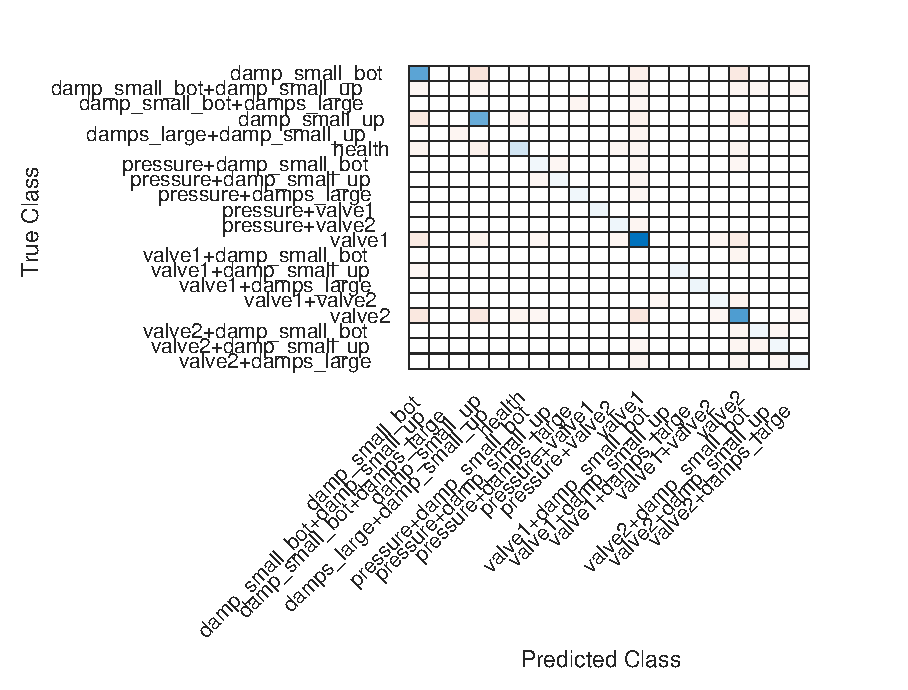
\includegraphics[width=\maxwidth{56.196688409433015em}]{figure_7.eps}
\end{center}
\begin{matlabcode}
reduced_features = acc_ranked_features.Features(1:50);
reduced_features_with_label = [reduced_features;"Label"];
reduced_features = features(:, reduced_features_with_label);
[train_data, test_data] = split_dataset(reduced_features);

[acc_model, ~ ] = acc_BaggedTrees_50_features_train(train_data);

acc_accuracy = confusion_matrix_plot_handler(acc_model, test_data);
\end{matlabcode}
\begin{matlaboutput}
Accuracy is 91.67 % 
\end{matlaboutput}
\begin{center}
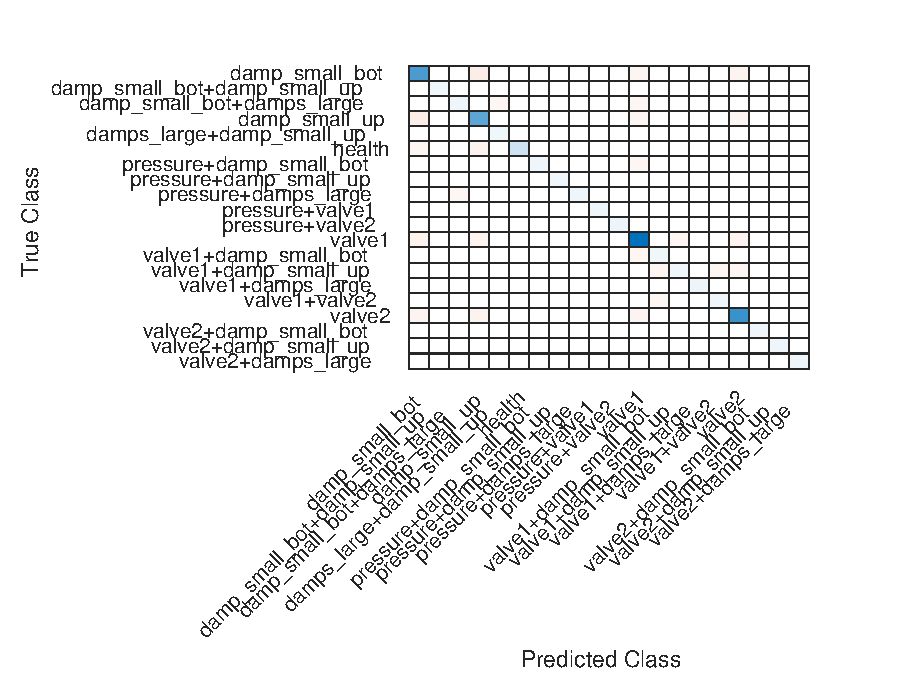
\includegraphics[width=\maxwidth{56.196688409433015em}]{figure_8.eps}
\end{center}

\label{H_03BE3A93}
\matlabheadingtwo{Conclusion}

\begin{matlabcode}
results_table.("Accelerometer") = table(acc_accuracy, acc_cost, acc_suitability, 'VariableNames', {'Perfomance', 'Cost', 'Suitability'});
\end{matlabcode}


\label{H_0F058F6E}
\matlabheading{Pressure Sensor}

\begin{matlabcode}
pressure_cost = 1000;
pressure_suitability = 0.5;

addpath("sensor_pressure/");
features = load("sensor_pressure/PressureAllFeatures.mat").PressureAllFeatures;

if compute_ranking
    [~,pressure_ranked_features,~] = pressure_features_process(features)
else
    pressure_ranked_features = load("sensor_pressure/pressure_ranked_features.mat").pressure_ranked_features
end
\end{matlabcode}
\begin{matlabtableoutput}
{
\begin{tabular} {|c|c|c|}\hline
\mlcell{ } & \mlcell{Features} & \mlcell{Kruskal-Wallis} \\ \hline
\mlcell{1} & \mlcell{"AirPressure\_stats/Std"} & \mlcell{1.1470e+03} \\ \hline
\mlcell{2} & \mlcell{"AirPressure\_stats/ShapeFactor"} & \mlcell{504.1080} \\ \hline
\mlcell{3} & \mlcell{"AirPressure\_stats/Kurtosis"} & \mlcell{321.8335} \\ \hline
\mlcell{4} & \mlcell{"AirPressure\_stats/PeakValue"} & \mlcell{249.0894} \\ \hline
\mlcell{5} & \mlcell{"AirPressure\_stats/SINAD"} & \mlcell{198.6519} \\ \hline
\mlcell{6} & \mlcell{"AirPressure\_stats/ClearanceFactor"} & \mlcell{172.6090} \\ \hline
\mlcell{7} & \mlcell{"AirPressure\_stats/RMS"} & \mlcell{164.2852} \\ \hline
\mlcell{8} & \mlcell{"AirPressure\_stats/ImpulseFactor"} & \mlcell{146.4968} \\ \hline
\mlcell{9} & \mlcell{"AirPressure\_stats/SNR"} & \mlcell{143.5568} \\ \hline
\mlcell{10} & \mlcell{"AirPressure\_stats/Mean"} & \mlcell{131.6099} \\ \hline
\mlcell{11} & \mlcell{"AirPressure\_stats/CrestFactor"} & \mlcell{128.4739} \\ \hline
\mlcell{12} & \mlcell{"AirPressure\_ps\_spec/BandPower"} & \mlcell{121.5916} \\ \hline
\mlcell{13} & \mlcell{"AirPressure\_ps\_spec/PeakAmp1"} & \mlcell{110.2916} \\ \hline
\mlcell{14} & \mlcell{"AirPressure\_stats/Skewness"} & \mlcell{102.7758} \\ \hline
\mlcell{15} & \mlcell{"AirPressure\_ps\_spec/PeakAmp6"} & \mlcell{100.3661} \\ \hline
\mlcell{16} & \mlcell{"AirPressure\_ps\_spec/PeakAmp7"} & \mlcell{77.7336} \\ \hline
\mlcell{17} & \mlcell{"AirPressure\_ps\_spec/PeakFreq6"} & \mlcell{75.7106} \\ \hline
\mlcell{18} & \mlcell{"AirPressure\_ps\_spec/PeakAmp8"} & \mlcell{62.6981} \\ \hline
\mlcell{19} & \mlcell{"AirPressure\_ps\_spec/PeakAmp5"} & \mlcell{52.8698} \\ \hline
\mlcell{20} & \mlcell{"AirPressure\_ps\_spec/PeakFreq4"} & \mlcell{51.5586} \\ \hline
\mlcell{21} & \mlcell{"AirPressure\_ps\_spec/PeakAmp2"} & \mlcell{51.2022} \\ \hline
\mlcell{22} & \mlcell{"AirPressure\_ps\_spec/PeakAmp3"} & \mlcell{47.1194} \\ \hline
\mlcell{23} & \mlcell{"AirPressure\_ps\_spec/PeakAmp4"} & \mlcell{44.9106} \\ \hline
\mlcell{24} & \mlcell{"AirPressure\_ps\_spec/PeakAmp9"} & \mlcell{37.9721} \\ \hline
\mlcell{25} & \mlcell{"AirPressure\_ps\_spec/PeakFreq3"} & \mlcell{35.7310} \\ \hline
\mlcell{26} & \mlcell{"AirPressure\_ps\_spec/PeakFreq7"} & \mlcell{24.9832} \\ \hline
\mlcell{27} & \mlcell{"AirPressure\_ps\_spec/PeakFreq9"} & \mlcell{23.2358} \\ \hline
\mlcell{28} & \mlcell{"AirPressure\_ps\_spec/PeakAmp10"} & \mlcell{19.9728} \\ \hline
\mlcell{29} & \mlcell{"AirPressure\_ps\_spec/PeakFreq10"} & \mlcell{12.6701} \\ \hline
\mlcell{30} & \mlcell{"AirPressure\_ps\_spec/PeakFreq2"} & \mlcell{11.4618} \\ \hline
\mlcell{31} & \mlcell{"AirPressure\_ps\_spec/PeakFreq5"} & \mlcell{9.8625} \\ \hline
\mlcell{32} & \mlcell{"AirPressure\_ps\_spec/PeakFreq8"} & \mlcell{9.6779} \\ \hline
\mlcell{33} & \mlcell{"AirPressure\_ps\_spec/PeakFreq1"} & \mlcell{1.3147} \\ \hline
\mlcell{34} & \mlcell{"AirPressure\_stats/THD"} & \mlcell{0} \\ 
\hline
\end{tabular}
}
\end{matlabtableoutput}

\begin{par}
\begin{flushleft}
Best result was achieved using all features without PCA.
\end{flushleft}
\end{par}

\begin{matlabcode}
[train_data, test_data] = split_dataset(features);
[pressure_model, ~ ] = pressure_BaggedTrees_AllFeatures_train(train_data);
pressure_accuracy = confusion_matrix_plot_handler(pressure_model, test_data);
\end{matlabcode}
\begin{matlaboutput}
Accuracy is 78.31 % 
\end{matlaboutput}
\begin{center}
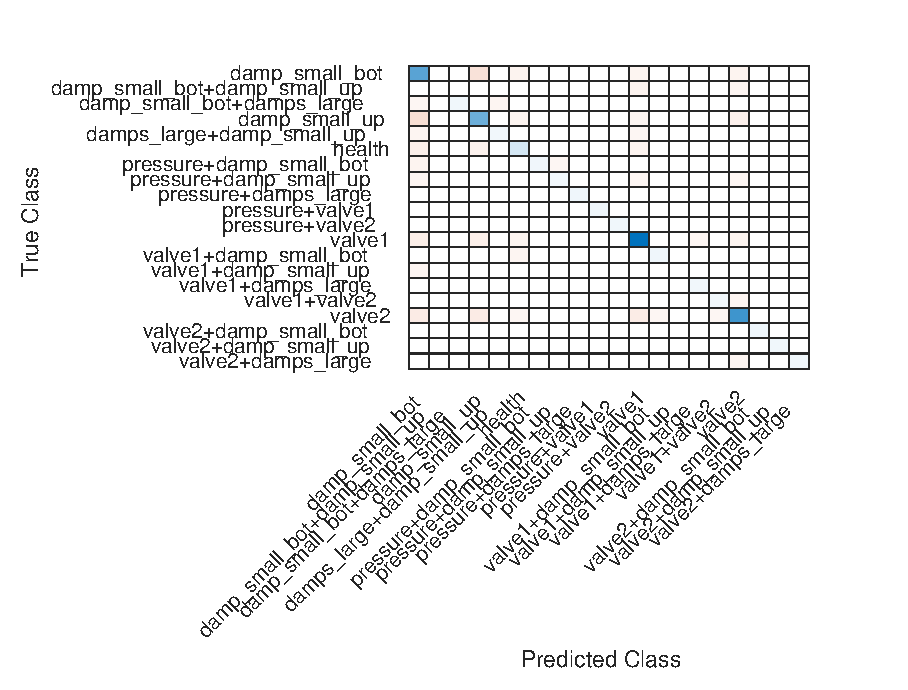
\includegraphics[width=\maxwidth{56.196688409433015em}]{figure_9.eps}
\end{center}

\label{H_1F1EF148}
\matlabheadingtwo{Conclusion}

\begin{matlabcode}
results_table.("Pressure") = table(pressure_accuracy, pressure_cost, pressure_suitability, 'VariableNames', {'Perfomance', 'Cost', 'Suitability'});
\end{matlabcode}


\label{H_CCEA380A}
\matlabheading{Proximity Sensors}

\begin{matlabcode}
proximity_cost = 1000*2;
proximity_suitability = 0.5;

addpath("sensor_proximity/");
features = load("sensor_proximity/ProximityAllFeatures.mat").ProximityAllFeatures;

if compute_ranking
    [~,proximity_ranked_features,~] = proximity_features_process(features)
else
    proximity_ranked_features = load("sensor_proximity/proximity_ranked_features.mat").proximity_ranked_features
end
\end{matlabcode}
\begin{matlabtableoutput}
{
\begin{tabular} {|c|c|c|}\hline
\mlcell{ } & \mlcell{Features} & \mlcell{Kruskal-Wallis} \\ \hline
\mlcell{1} & \mlcell{"ProximitySensor\_bottom\_stats/SINAD"} & \mlcell{NaN} \\ \hline
\mlcell{2} & \mlcell{"ProximitySensor\_bottom\_stats/SNR"} & \mlcell{NaN} \\ \hline
\mlcell{3} & \mlcell{"ProximitySensor\_bottom\_stats/THD"} & \mlcell{NaN} \\ \hline
\mlcell{4} & \mlcell{"ProximitySensor\_bottom\_stats/ClearanceFactor"} & \mlcell{654.5551} \\ \hline
\mlcell{5} & \mlcell{"ProximitySensor\_bottom\_stats/CrestFactor"} & \mlcell{654.5551} \\ \hline
\mlcell{6} & \mlcell{"ProximitySensor\_bottom\_stats/ImpulseFactor"} & \mlcell{654.5551} \\ \hline
\mlcell{7} & \mlcell{"ProximitySensor\_bottom\_stats/ShapeFactor"} & \mlcell{654.5551} \\ \hline
\mlcell{8} & \mlcell{"ProximitySensor\_bottom\_stats/Skewness"} & \mlcell{654.5344} \\ \hline
\mlcell{9} & \mlcell{"ProximitySensor\_bottom\_stats/Kurtosis"} & \mlcell{606.4626} \\ \hline
\mlcell{10} & \mlcell{"ProximitySensor\_bottom\_stats/Mean"} & \mlcell{601.0174} \\ \hline
\mlcell{11} & \mlcell{"ProximitySensor\_bottom\_stats/RMS"} & \mlcell{601.0174} \\ \hline
\mlcell{12} & \mlcell{"ProximitySensor\_bottom\_stats/Std"} & \mlcell{552.1008} \\ \hline
\mlcell{13} & \mlcell{"ProximitySensor\_upper\_stats/PeakValue"} & \mlcell{469.0708} \\ \hline
\mlcell{14} & \mlcell{"ProximitySensor\_upper\_stats/Std"} & \mlcell{455.4724} \\ \hline
\mlcell{15} & \mlcell{"ProximitySensor\_upper\_stats/Mean"} & \mlcell{455.4640} \\ \hline
\mlcell{16} & \mlcell{"ProximitySensor\_upper\_stats/RMS"} & \mlcell{455.4640} \\ \hline
\mlcell{17} & \mlcell{"ProximitySensor\_upper\_stats/SINAD"} & \mlcell{354.6982} \\ \hline
\mlcell{18} & \mlcell{"ProximitySensor\_upper\_stats/Skewness"} & \mlcell{332.1729} \\ \hline
\mlcell{19} & \mlcell{"ProximitySensor\_upper\_stats/Kurtosis"} & \mlcell{332.1729} \\ \hline
\mlcell{20} & \mlcell{"ProximitySensor\_upper\_stats/ClearanceFactor"} & \mlcell{332.1664} \\ \hline
\mlcell{21} & \mlcell{"ProximitySensor\_upper\_stats/CrestFactor"} & \mlcell{332.1664} \\ \hline
\mlcell{22} & \mlcell{"ProximitySensor\_upper\_stats/ImpulseFactor"} & \mlcell{332.1664} \\ \hline
\mlcell{23} & \mlcell{"ProximitySensor\_upper\_stats/ShapeFactor"} & \mlcell{332.1664} \\ \hline
\mlcell{24} & \mlcell{"ProximitySensor\_bottom\_stats/PeakValue"} & \mlcell{320.9818} \\ \hline
\mlcell{25} & \mlcell{"ProximitySensor\_upper\_stats/SNR"} & \mlcell{319.3780} \\ \hline
\mlcell{26} & \mlcell{"ProximitySensor\_upper\_stats/THD"} & \mlcell{314.5699} \\ 
\hline
\end{tabular}
}
\end{matlabtableoutput}

\begin{par}
\begin{flushleft}
Best result was achieved using all features without PCA.
\end{flushleft}
\end{par}

\begin{matlabcode}
[train_data, test_data] = split_dataset(features);

[proximity_model, ~ ] = proximity_BaggedTrees_AllFeatures_train(train_data);

proximity_accuracy = confusion_matrix_plot_handler(proximity_model, test_data);
\end{matlabcode}
\begin{matlaboutput}
Accuracy is 87.33 % 
\end{matlaboutput}
\begin{center}
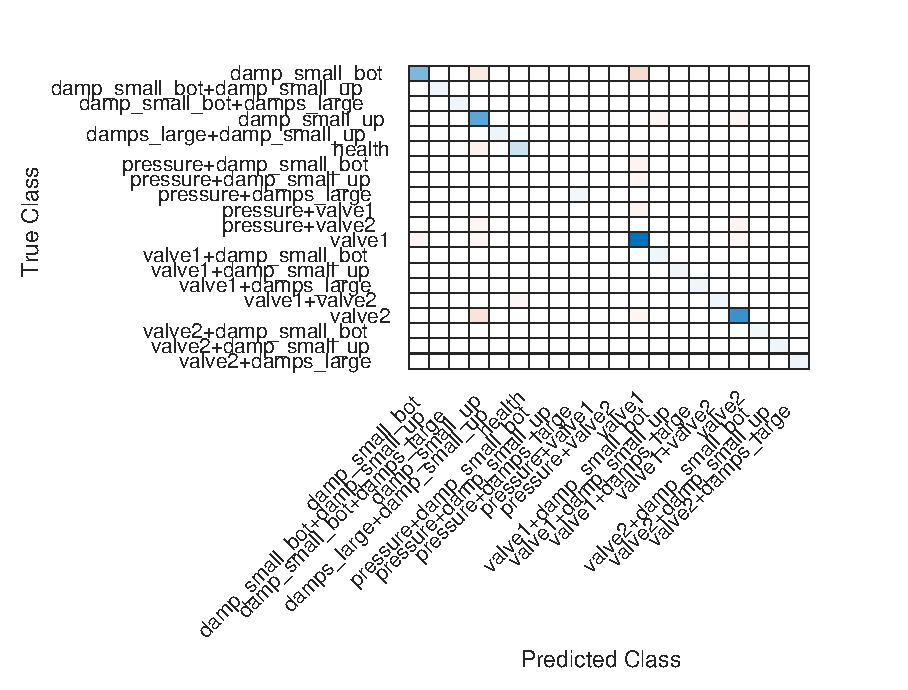
\includegraphics[width=\maxwidth{56.196688409433015em}]{figure_10.eps}
\end{center}

\label{H_E5CB5CAB}
\matlabheadingtwo{Conclusion}

\begin{matlabcode}
results_table.("Proximity") = table(proximity_accuracy, proximity_cost, proximity_suitability, 'VariableNames', {'Perfomance', 'Cost', 'Suitability'});
\end{matlabcode}


\label{H_C3A12018}
\matlabheading{Strain Gauge}

\begin{matlabcode}
straingauge_cost = 15000;
straingauge_suitability = 0.5;

addpath("sensor_strain/");
features = load("sensor_strain/StrainAllFeatures.mat").StrainAllFeatures;

if compute_ranking
    [~,strain_ranked_features,~] = strain_features_process(features)
else
    strain_ranked_features = load("sensor_strain/strain_ranked_features.mat").strain_ranked_features
end
\end{matlabcode}
\begin{matlabtableoutput}
{
\begin{tabular} {|c|c|c|}\hline
\mlcell{ } & \mlcell{Features} & \mlcell{Kruskal-Wallis} \\ \hline
\mlcell{1} & \mlcell{"StrainGauge\_stats/ClearanceFactor"} & \mlcell{821.7769} \\ \hline
\mlcell{2} & \mlcell{"StrainGauge\_stats/SNR"} & \mlcell{550.9483} \\ \hline
\mlcell{3} & \mlcell{"StrainGauge\_stats/ShapeFactor"} & \mlcell{393.5707} \\ \hline
\mlcell{4} & \mlcell{"StrainGauge\_stats/Std"} & \mlcell{345.1350} \\ \hline
\mlcell{5} & \mlcell{"StrainGauge\_stats/ImpulseFactor"} & \mlcell{333.9208} \\ \hline
\mlcell{6} & \mlcell{"StrainGauge\_stats/Kurtosis"} & \mlcell{284.4512} \\ \hline
\mlcell{7} & \mlcell{"StrainGauge\_stats/SINAD"} & \mlcell{279.3896} \\ \hline
\mlcell{8} & \mlcell{"StrainGauge\_ps\_spec/PeakAmp3"} & \mlcell{275.8916} \\ \hline
\mlcell{9} & \mlcell{"StrainGauge\_ps\_spec/BandPower"} & \mlcell{265.1367} \\ \hline
\mlcell{10} & \mlcell{"StrainGauge\_stats/CrestFactor"} & \mlcell{257.8783} \\ \hline
\mlcell{11} & \mlcell{"StrainGauge\_ps\_spec/PeakAmp1"} & \mlcell{234.8921} \\ \hline
\mlcell{12} & \mlcell{"StrainGauge\_stats/RMS"} & \mlcell{211.7432} \\ \hline
\mlcell{13} & \mlcell{"StrainGauge\_stats/Mean"} & \mlcell{205.2573} \\ \hline
\mlcell{14} & \mlcell{"StrainGauge\_ps\_spec/PeakAmp4"} & \mlcell{188.9729} \\ \hline
\mlcell{15} & \mlcell{"StrainGauge\_ps\_spec/PeakAmp9"} & \mlcell{157.8649} \\ \hline
\mlcell{16} & \mlcell{"StrainGauge\_stats/PeakValue"} & \mlcell{149.6731} \\ \hline
\mlcell{17} & \mlcell{"StrainGauge\_ps\_spec/PeakAmp8"} & \mlcell{139.8552} \\ \hline
\mlcell{18} & \mlcell{"StrainGauge\_ps\_spec/PeakAmp2"} & \mlcell{134.6385} \\ \hline
\mlcell{19} & \mlcell{"StrainGauge\_ps\_spec/PeakAmp6"} & \mlcell{129.8935} \\ \hline
\mlcell{20} & \mlcell{"StrainGauge\_ps\_spec/PeakFreq3"} & \mlcell{124.3427} \\ \hline
\mlcell{21} & \mlcell{"StrainGauge\_ps\_spec/PeakFreq4"} & \mlcell{118.6774} \\ \hline
\mlcell{22} & \mlcell{"StrainGauge\_ps\_spec/PeakAmp7"} & \mlcell{108.2226} \\ \hline
\mlcell{23} & \mlcell{"StrainGauge\_stats/Skewness"} & \mlcell{100.6661} \\ \hline
\mlcell{24} & \mlcell{"StrainGauge\_ps\_spec/PeakAmp10"} & \mlcell{96.6493} \\ \hline
\mlcell{25} & \mlcell{"StrainGauge\_ps\_spec/PeakAmp5"} & \mlcell{90.7219} \\ \hline
\mlcell{26} & \mlcell{"StrainGauge\_ps\_spec/PeakFreq5"} & \mlcell{86.6373} \\ \hline
\mlcell{27} & \mlcell{"StrainGauge\_ps\_spec/PeakFreq6"} & \mlcell{78.0176} \\ \hline
\mlcell{28} & \mlcell{"StrainGauge\_stats/THD"} & \mlcell{75.3171} \\ \hline
\mlcell{29} & \mlcell{"StrainGauge\_ps\_spec/PeakFreq2"} & \mlcell{62.9067} \\ \hline
\mlcell{30} & \mlcell{"StrainGauge\_ps\_spec/PeakFreq9"} & \mlcell{60.5085} \\ \hline
\mlcell{31} & \mlcell{"StrainGauge\_ps\_spec/PeakFreq7"} & \mlcell{58.5055} \\ \hline
\mlcell{32} & \mlcell{"StrainGauge\_ps\_spec/PeakFreq8"} & \mlcell{50.1456} \\ \hline
\mlcell{33} & \mlcell{"StrainGauge\_ps\_spec/PeakFreq10"} & \mlcell{47.9735} \\ \hline
\mlcell{34} & \mlcell{"StrainGauge\_ps\_spec/PeakFreq1"} & \mlcell{1.3156} \\ 
\hline
\end{tabular}
}
\end{matlabtableoutput}
\begin{matlabcode}
reduced_features = strain_ranked_features.Features(1:5);
reduced_features_with_label = [reduced_features;"Label"];
reduced_features = features(:, reduced_features_with_label);
[train_data, test_data] = split_dataset(reduced_features);

[strain_model, ~ ] = strain_BaggedTrees_anova_train(train_data);

straingauge_accuracy = confusion_matrix_plot_handler(strain_model, test_data);
\end{matlabcode}
\begin{matlaboutput}
Accuracy is 95.39 % 
\end{matlaboutput}
\begin{center}
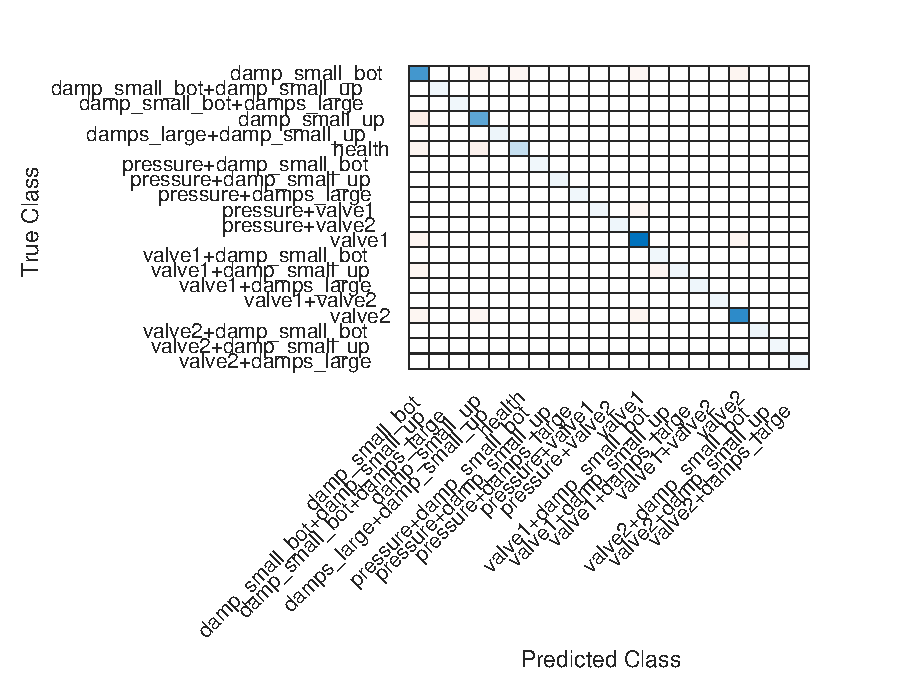
\includegraphics[width=\maxwidth{56.196688409433015em}]{figure_11.eps}
\end{center}

\label{H_B0AA0DEB}
\matlabheadingtwo{Conclusion}

\begin{matlabcode}
results_table.("Strain") = table(straingauge_accuracy, straingauge_cost, straingauge_suitability, 'VariableNames', {'Perfomance', 'Cost', 'Suitability'});
\end{matlabcode}


\label{H_BABF6AEB}
\matlabheading{Temperature Sensors}

\begin{par}
\begin{flushleft}
Temperature sensors do only one measurement during the experiment. 
\end{flushleft}
\end{par}

\begin{par}
\begin{flushleft}
These values can be represented as features. Plotting random data from the dataset shows that they correlated to Ambient temperature different in different measurement days. These data are sensitive to ambient conditions. The classification model trained on this data not robust in real life.
\end{flushleft}
\end{par}

\begin{matlabcode}
temp_features = load("featuretable/temp_features.mat").temp_features;
figure
hold on
for i = 1:size(temp_features)
    var = temp_features(i,:);
    label = var.Label;
    temp_cylinder = var.Temp_Cylinder;
    temp_ambient = var.Temp_Ambient;
    switch label
        case "health"
            plot(temp_cylinder, temp_ambient, 'r.')
        case "valve1"
            plot(temp_cylinder, temp_ambient, 'g.')
        case "valve2"
            plot(temp_cylinder, temp_ambient, 'b.')
        case "damp_small_bot"
            plot(temp_cylinder, temp_ambient, 'k.')
        case "damp_small_up"
            plot(temp_cylinder, temp_ambient, 'y.')
    end
end
title("Temperature Cylinder vs Temperature Ambient")
xlabel("Temperature Cylinder [C]")
ylabel("Temperature Ambient [C]")
\end{matlabcode}
\begin{center}
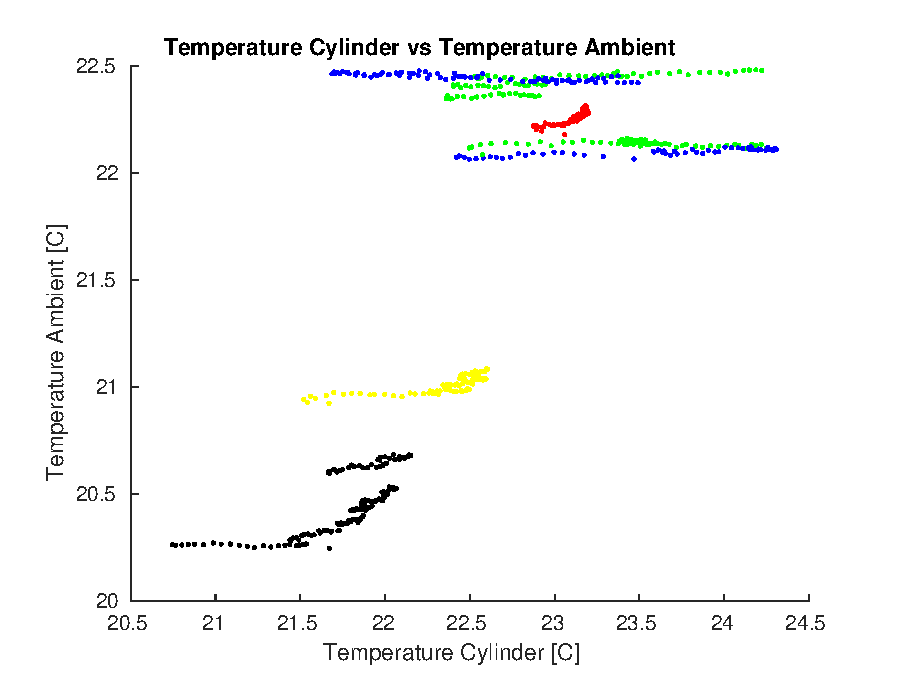
\includegraphics[width=\maxwidth{56.196688409433015em}]{figure_12.eps}
\end{center}


\label{H_16C31A77}
\matlabheading{Conclusion}

\begin{matlabcode}
result_table = struct2table(results_table);
sensors_efficiency = table();
perf_coef = 1;  % TODO
cost_coef = 1;  % TODO
suit_coef = 1;  % TODO

for sensor = result_table.Properties.VariableNames
    disp(string(sensor))
    var = result_table.(string(sensor))
    sensors_efficiency.(string(sensor)) = perf_coef*var.Perfomance+cost_coef*var.Cost+suit_coef*var.Suitability;
end
\end{matlabcode}
\begin{matlaboutput}
Encoder
\end{matlaboutput}
\begin{matlabtableoutput}
{
\begin{tabular} {|c|c|c|c|}\hline
\mlcell{ } & \mlcell{Perfomance} & \mlcell{Cost} & \mlcell{Suitability} \\ \hline
\mlcell{1} & \mlcell{0.9725} & \mlcell{25000} & \mlcell{0.1000} \\ 
\hline
\end{tabular}
}
\end{matlabtableoutput}
\begin{matlaboutput}
Mics
\end{matlaboutput}
\begin{matlabtableoutput}
{
\begin{tabular} {|c|c|c|c|}\hline
\mlcell{ } & \mlcell{Perfomance} & \mlcell{Cost} & \mlcell{Suitability} \\ \hline
\mlcell{1} & \mlcell{0.9477} & \mlcell{1500} & \mlcell{1} \\ 
\hline
\end{tabular}
}
\end{matlabtableoutput}
\begin{matlaboutput}
Flow
\end{matlaboutput}
\begin{matlabtableoutput}
{
\begin{tabular} {|c|c|c|c|}\hline
\mlcell{ } & \mlcell{Perfomance} & \mlcell{Cost} & \mlcell{Suitability} \\ \hline
\mlcell{1} & \mlcell{0.9711} & \mlcell{12000} & \mlcell{0.5000} \\ 
\hline
\end{tabular}
}
\end{matlabtableoutput}
\begin{matlaboutput}
Accelerometer
\end{matlaboutput}
\begin{matlabtableoutput}
{
\begin{tabular} {|c|c|c|c|}\hline
\mlcell{ } & \mlcell{Perfomance} & \mlcell{Cost} & \mlcell{Suitability} \\ \hline
\mlcell{1} & \mlcell{0.9167} & \mlcell{7000} & \mlcell{0.5000} \\ 
\hline
\end{tabular}
}
\end{matlabtableoutput}
\begin{matlaboutput}
Pressure
\end{matlaboutput}
\begin{matlabtableoutput}
{
\begin{tabular} {|c|c|c|c|}\hline
\mlcell{ } & \mlcell{Perfomance} & \mlcell{Cost} & \mlcell{Suitability} \\ \hline
\mlcell{1} & \mlcell{0.7831} & \mlcell{1000} & \mlcell{0.5000} \\ 
\hline
\end{tabular}
}
\end{matlabtableoutput}
\begin{matlaboutput}
Proximity
\end{matlaboutput}
\begin{matlabtableoutput}
{
\begin{tabular} {|c|c|c|c|}\hline
\mlcell{ } & \mlcell{Perfomance} & \mlcell{Cost} & \mlcell{Suitability} \\ \hline
\mlcell{1} & \mlcell{0.8733} & \mlcell{2000} & \mlcell{0.5000} \\ 
\hline
\end{tabular}
}
\end{matlabtableoutput}
\begin{matlaboutput}
Strain
\end{matlaboutput}
\begin{matlabtableoutput}
{
\begin{tabular} {|c|c|c|c|}\hline
\mlcell{ } & \mlcell{Perfomance} & \mlcell{Cost} & \mlcell{Suitability} \\ \hline
\mlcell{1} & \mlcell{0.9539} & \mlcell{15000} & \mlcell{0.5000} \\ 
\hline
\end{tabular}
}
\end{matlabtableoutput}
\begin{matlabcode}
sensors_efficiency
\end{matlabcode}
\begin{matlabtableoutput}
{
\begin{tabular} {|c|c|c|c|c|c|c|c|}\hline
\mlcell{ } & \mlcell{Encoder} & \mlcell{Mics} & \mlcell{Flow} & \mlcell{Accelerometer} & \mlcell{Pressure} & \mlcell{Proximity} & \mlcell{Strain} \\ \hline
\mlcell{1} & \mlcell{2.5001e+04} & \mlcell{1.5019e+03} & \mlcell{1.2001e+04} & \mlcell{7.0014e+03} & \mlcell{1.0013e+03} & \mlcell{2.0014e+03} & \mlcell{1.5001e+04} \\ 
\hline
\end{tabular}
}
\end{matlabtableoutput}
\begin{matlabcode}

x = [];
y1 = [];
y2 = [];
for sensor = result_table.Properties.VariableNames
    x = [x string(sensor)];
    var = result_table.(string(sensor));
    y1 = [y1;var.Perfomance];
    y2 = [y2;var.Cost];
end
x = categorical(x');
y1 = double([y1 zeros(7,1)])*100;
y2 = double([zeros(7,1) y2]);

figure
hold on
yyaxis left
b1 = bar(x,y1);
ylabel("Accuracy in %", 'Color', 'k')

yyaxis right
b2 = bar(x,y2);
ylabel("Cost [czk]", 'Color', 'k')
hold off
title("Comparison of sensors")
\end{matlabcode}
\begin{center}
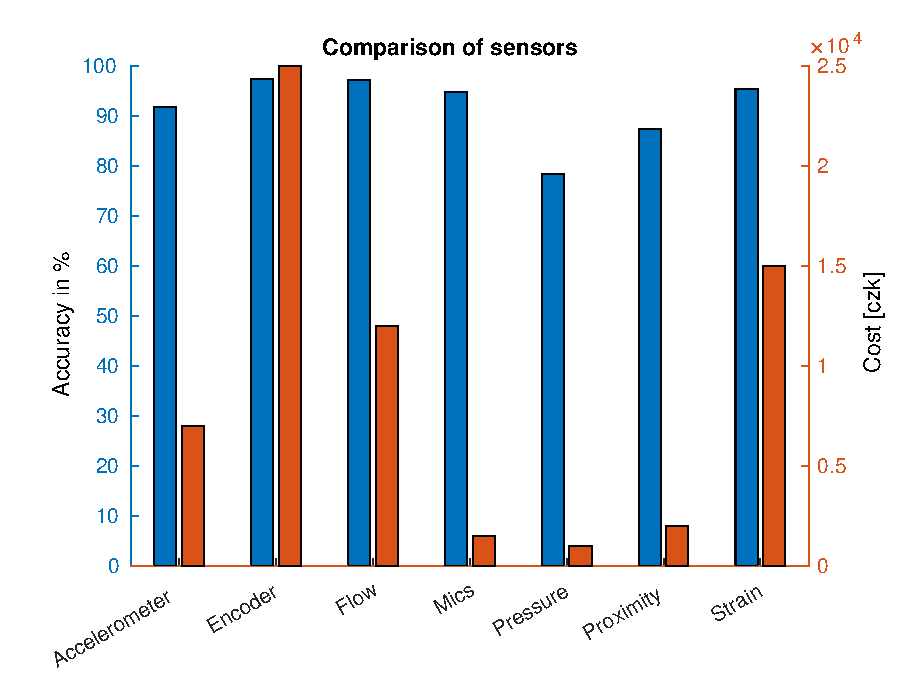
\includegraphics[width=\maxwidth{56.196688409433015em}]{figure_13.eps}
\end{center}


\begin{matlabcode}
function [dataTrain, dataTest] = split_dataset(data)
    cv = cvpartition(size(data,1), 'HoldOut', 0.3);
    idx = cv.test;      
    dataTrain = data(~idx, :);
    dataTest = data(idx, :);
end

function [accuracy] = confusion_matrix_plot_handler(mdl, features)
    required_features = mdl.RequiredVariables;
    targetLabels = features(:,"Label");
    inputTable = features(:, required_features);
    predictedLabels = mdl.predictFcn(inputTable);
    [C,order] = confusionmat(table2array(targetLabels),predictedLabels);
    accuracy = sum(table2array(targetLabels) == predictedLabels)/numel(predictedLabels);
    fprintf("Accuracy is %0.2f %% \n", accuracy*100)
    figure
    confusionchart(C, order)
end
\end{matlabcode}

\end{document}
